\documentclass[11pt,a4paper]{article}
\usepackage[utf8]{inputenc}
\usepackage[T1]{fontenc}
\usepackage[brazil]{babel}
\usepackage{amsmath,amssymb,amsthm}
\usepackage{bm}
\usepackage{booktabs}
\usepackage{graphicx}
\usepackage{geometry}
\usepackage{hyperref}
\usepackage{float}

\geometry{margin=2.2cm}
\hypersetup{colorlinks=true, linkcolor=blue, urlcolor=blue}

\title{\textbf{Projeto Final — Álgebra Linear e Otimização para Aprendizado de Máquina}\\
\large Relatório Técnico Completo e Memorial de Cálculo Analítico}
\author{
Integrante 1 (RA: \textit{a preencher}) \and
Integrante 2 (RA: \textit{a preencher}) \and
Integrante 3 (RA: \textit{opcional})
}
\date{Instituto de Computação — UNICAMP \\ 2º Semestre de 2026}

\begin{document}
\maketitle

\begin{abstract}
Este relatório técnico apresenta o memorial de cálculo analítico passo a passo, todas as matrizes intermediárias, demonstrações formais e validações numéricas em \texttt{numpy} puro para as Questões 1 a 6 e Questão Bônus do Projeto Final da disciplina \textit{Álgebra Linear e Otimização para Aprendizado de Máquina} (IC/UNICAMP). Todas as identidades algébricas e taxas de convergência foram verificadas computacionalmente dentro de tolerâncias de ponto flutuante entre $10^{-10}$ e $10^{-15}$, com semente aleatória fixada (\texttt{np.random.seed(42)}).
\end{abstract}

\tableofcontents
\newpage

% ==============================================================================
\section{Questão 1: Normas, Métricas, Escala e o Algoritmo $k$-NN}
% ==============================================================================

\subsection{Parte A: Normas, Métricas e Impacto de Escala}

\subsubsection*{A.1. Cálculo Analítico das Distâncias sob as Normas $L_1$, $L_2$ e $L_\infty$}
Dado o ponto de consulta $\mathbf{x}_{\text{novo}} = [6{,}0 \quad 20{,}0]^T \in \mathbb{R}^2$ e cada amostra $\mathbf{x}_i = [x_{i1} \quad x_{i2}]^T$ do Dataset $\mathcal{D}$, definimos o vetor diferença $\boldsymbol{\delta}_i = \mathbf{x}_i - \mathbf{x}_{\text{novo}} = [\Delta x_{i1} \quad \Delta x_{i2}]^T$:
\begin{itemize}
    \item \textbf{Norma $L_1$ (Manhattan):} $d_1(\mathbf{x}_i, \mathbf{x}_{\text{novo}}) = |\Delta x_{i1}| + |\Delta x_{i2}|$.
    \item \textbf{Norma $L_2$ (Euclidiana):} $d_2(\mathbf{x}_i, \mathbf{x}_{\text{novo}}) = \sqrt{(\Delta x_{i1})^2 + (\Delta x_{i2})^2}$.
    \item \textbf{Norma $L_\infty$ (Chebyshev/Máximo):} $d_\infty(\mathbf{x}_i, \mathbf{x}_{\text{novo}}) = \max(|\Delta x_{i1}|, |\Delta x_{i2}|)$.
\end{itemize}

Desenvolvimento analítico amostra por amostra:
\begin{enumerate}
    \item \textbf{Amostra 1 ($\mathbf{x}_1 = [5{,}0, 30{,}0]^T$):} $\boldsymbol{\delta}_1 = [-1{,}0, 10{,}0]^T \implies d_1 = 1{,}0 + 10{,}0 = 11{,}0$; $d_2 = \sqrt{(-1{,}0)^2 + 10{,}0^2} = \sqrt{101} \approx 10{,}049876$; $d_\infty = \max(1{,}0, 10{,}0) = 10{,}0$.
    \item \textbf{Amostra 2 ($\mathbf{x}_2 = [7{,}0, 38{,}0]^T$):} $\boldsymbol{\delta}_2 = [1{,}0, 18{,}0]^T \implies d_1 = 1{,}0 + 18{,}0 = 19{,}0$; $d_2 = \sqrt{1{,}0^2 + 18{,}0^2} = \sqrt{325} = 5\sqrt{13} \approx 18{,}027756$; $d_\infty = \max(1{,}0, 18{,}0) = 18{,}0$.
    \item \textbf{Amostra 3 ($\mathbf{x}_3 = [9{,}0, 40{,}0]^T$):} $\boldsymbol{\delta}_3 = [3{,}0, 20{,}0]^T \implies d_1 = 3{,}0 + 20{,}0 = 23{,}0$; $d_2 = \sqrt{3{,}0^2 + 20{,}0^2} = \sqrt{409} \approx 20{,}223748$; $d_\infty = \max(3{,}0, 20{,}0) = 20{,}0$.
    \item \textbf{Amostra 4 ($\mathbf{x}_4 = [3{,}5, 19{,}0]^T$):} $\boldsymbol{\delta}_4 = [-2{,}5, -1{,}0]^T \implies d_1 = 2{,}5 + 1{,}0 = 3{,}5$; $d_2 = \sqrt{(-2{,}5)^2 + (-1{,}0)^2} = \sqrt{7{,}25} = \frac{\sqrt{29}}{2} \approx 2{,}692582$; $d_\infty = \max(2{,}5, 1{,}0) = 2{,}5$.
    \item \textbf{Amostra 5 ($\mathbf{x}_5 = [8{,}0, 15{,}0]^T$):} $\boldsymbol{\delta}_5 = [2{,}0, -5{,}0]^T \implies d_1 = 2{,}0 + 5{,}0 = 7{,}0$; $d_2 = \sqrt{2{,}0^2 + (-5{,}0)^2} = \sqrt{29} \approx 5{,}385165$; $d_\infty = \max(2{,}0, 5{,}0) = 5{,}0$.
    \item \textbf{Amostra 6 ($\mathbf{x}_6 = [2{,}0, 35{,}0]^T$):} $\boldsymbol{\delta}_6 = [-4{,}0, 15{,}0]^T \implies d_1 = 4{,}0 + 15{,}0 = 19{,}0$; $d_2 = \sqrt{(-4{,}0)^2 + 15{,}0^2} = \sqrt{241} \approx 15{,}524175$; $d_\infty = \max(4{,}0, 15{,}0) = 15{,}0$.
\end{enumerate}

\begin{table}[H]
\centering
\caption{Distâncias exatas de cada amostra de $\mathcal{D}$ até $\mathbf{x}_{\text{novo}} = [6{,}0, 20{,}0]^T$ e rankings induzidos.}
\label{tab:q1_dists}
\begin{tabular}{ccccccc}
\toprule
Amostra & $d_1$ (Rank) & $d_2$ (Rank) & $d_\infty$ (Rank) & $d_2^{(z)}$ Z-Score (Rank) & Mahalanobis (Rank) & $(y_i, c_i)$ \\
\midrule
1 & $11{,}0$ (3º) & $\sqrt{101} \approx 10{,}0499$ (3º) & $10{,}0$ (3º) & $1{,}0358$ (3º) & $1{,}0773$ (3º) & $(2{,}5, 0)$ \\
2 & $19{,}0$ (4º/5º) & $\sqrt{325} \approx 18{,}0278$ (5º) & $18{,}0$ (5º) & $1{,}7811$ (4º) & $1{,}7525$ (4º) & $(3{,}8, 0)$ \\
3 & $23{,}0$ (6º) & $\sqrt{409} \approx 20{,}2237$ (6º) & $20{,}0$ (6º) & $2{,}2292$ (6º) & $2{,}1377$ (5º) & $(4{,}2, 1)$ \\
4 & $3{,}5$ (1º) & $\sqrt{7{,}25} \approx 2{,}6926$ (1º) & $2{,}5$ (1º) & $0{,}9257$ (2º) & $0{,}9206$ (1º) & $(1{,}9, 0)$ \\
5 & $7{,}0$ (2º) & $\sqrt{29} \approx 5{,}3852$ (2º) & $5{,}0$ (2º) & $0{,}8813$ (1º) & $0{,}9280$ (2º) & $(4{,}5, 1)$ \\
6 & $19{,}0$ (4º/5º) & $\sqrt{241} \approx 15{,}5242$ (4º) & $15{,}0$ (4º) & $2{,}0684$ (5º) & $2{,}1865$ (6º) & $(1{,}2, 0)$ \\
\bottomrule
\end{tabular}
\end{table}

\subsubsection*{A.2. Impacto da Escala e Geometria das Bolas Métricas}
Sim, a escala dos atributos afeta criticamente as distâncias. No Dataset $\mathcal{D}$, $x_1$ (área) varia em $[2{,}0, 9{,}0]$ (variância amostral $s_1^2 = 7{,}375$), enquanto $x_2$ (idade) varia em $[15{,}0, 40{,}0]$ (variância amostral $s_2^2 = 106{,}70$, ou seja, $14{,}47\times$ maior). Expressando as diferenças em coordenadas padronizadas $\Delta z_j = \Delta x_j / \sigma_j$, a condição da bola euclidiana bruta $\|\mathbf{x} - \mathbf{x}_{\text{novo}}\|_2 \le r$ reescreve-se como:
\[
\sigma_1^2 (\Delta z_1)^2 + \sigma_2^2 (\Delta z_2)^2 \le r^2 \iff \frac{(\Delta z_1)^2}{(r/\sigma_1)^2} + \frac{(\Delta z_2)^2}{(r/\sigma_2)^2} \le 1.
\]
Como $\sigma_2 \gg \sigma_1$, o círculo bruto mapeia-se em uma \textbf{elipse severamente achatada na direção da idade ($z_2$) e alongada na direção da área ($z_1$)}. Assim, diferenças em anos dominam o cálculo da distância e obscurecem variações na área. Após padronização Z-score (\texttt{ddof=1}, com $\boldsymbol{\mu} = [5{,}75, 29{,}50]^T$ e $\boldsymbol{\sigma} \approx [2{,}7157, 10{,}3296]^T$), o 1º vizinho mais próximo inverte-se da Amostra 4 ($c_4=0, d_2^{(z)} = 0{,}9257$) para a Amostra 5 ($c_5=1, d_2^{(z)} = 0{,}8813$), alterando diretamente a decisão do classificador $1$-NN.

\subsubsection*{A.3. Contraexemplo Formal: Dissimilaridade do Cosseno não é Métrica}
Para $d_{\cos}(\mathbf{u}, \mathbf{v}) = 1 - \frac{\langle \mathbf{u}, \mathbf{v} \rangle}{\|\mathbf{u}\|_2 \|\mathbf{v}\|_2}$, uma métrica formal exige a desigualdade triangular $d_{\cos}(\mathbf{u}, \mathbf{w}) \le d_{\cos}(\mathbf{u}, \mathbf{v}) + d_{\cos}(\mathbf{v}, \mathbf{w})$. Sejam três vetores unitários em $\mathbb{R}^2$:
\[
\mathbf{u} = \begin{bmatrix} 1 \\ 0 \end{bmatrix}, \qquad
\mathbf{v} = \begin{bmatrix} \frac{\sqrt{2}}{2} \\ \frac{\sqrt{2}}{2} \end{bmatrix} \text{ ($45^\circ$)}, \qquad
\mathbf{w} = \begin{bmatrix} 0 \\ 1 \end{bmatrix} \text{ ($90^\circ$)}.
\]
Calculando os três valores:
\[
d_{\cos}(\mathbf{u}, \mathbf{v}) = 1 - \frac{\sqrt{2}}{2} \approx 0{,}292893, \quad
d_{\cos}(\mathbf{v}, \mathbf{w}) = 1 - \frac{\sqrt{2}}{2} \approx 0{,}292893, \quad
d_{\cos}(\mathbf{u}, \mathbf{w}) = 1 - 0 = 1{,}0.
\]
Somando os dois primeiros: $d_{\cos}(\mathbf{u}, \mathbf{v}) + d_{\cos}(\mathbf{v}, \mathbf{w}) = 2 - \sqrt{2} \approx 0{,}585786 < 1{,}0 = d_{\cos}(\mathbf{u}, \mathbf{w})$. Logo, a desigualdade triangular é estritamente violada, provando que $d_{\cos}$ não é uma métrica formal.

\subsection{Parte B: Algoritmo $k$-NN e Hipótese de Suavidade}

\subsubsection*{B.1. Predições sob Distância Euclidiana ($L_2$) Bruta}
Pela Tabela~\ref{tab:q1_dists}, os três vizinhos mais próximos de $\mathbf{x}_{\text{novo}}$ são $\{4, 5, 1\}$:
\begin{itemize}
    \item \textbf{Classificação $k=1$:} $\mathcal{N}_1 = \{4\} \implies \hat{c}_{\text{novo}}^{(1)} = c_4 = 0$.
    \item \textbf{Classificação $k=3$:} $\mathcal{N}_3 = \{4, 5, 1\}$ com rótulos $\{0, 1, 0\} \implies$ por voto majoritário (2 contra 1), $\hat{c}_{\text{novo}}^{(3)} = 0$.
    \item \textbf{Regressão $k=3$:} média aritmética dos alvos $\hat{y}_{\text{novo}}^{(3)} = \frac{y_4 + y_5 + y_1}{3} = \frac{1{,}9 + 4{,}5 + 2{,}5}{3} = \frac{8{,}9}{3} \approx 2{,}966667$.
\end{itemize}

\subsubsection*{B.2. Hipótese de Suavidade e Compromisso Viés-Variância ($k=1$ vs. $k=N=6$)}
O algoritmo $k$-NN apoia-se na \textbf{hipótese de suavidade local} (\textit{smoothness assumption}): pontos próximos no espaço métrico compartilham valores semelhantes de $\mathbb{E}[Y \mid \mathbf{X}=\mathbf{x}]$. Sob $y_i = f(\mathbf{x}_i) + \varepsilon_i$ com $\operatorname{Var}(\varepsilon_i) = \sigma_\varepsilon^2$, o erro quadrático médio de $\hat{f}_k(\mathbf{x})$ decompõe-se em:
\[
\operatorname{MSE}(\hat{f}_k(\mathbf{x})) = \underbrace{\left(f(\mathbf{x}) - \frac{1}{k}\sum_{i \in \mathcal{N}_k(\mathbf{x})} f(\mathbf{x}_i)\right)^2}_{\text{Viés}^2} + \underbrace{\frac{\sigma_\varepsilon^2}{k}}_{\text{Variância}} + \sigma_\varepsilon^2.
\]
\begin{itemize}
    \item \textbf{Extremo $k=1$:} Baixíssimo viés local (usa apenas o vizinho mais próximo), mas variância máxima ($\sigma_\varepsilon^2$). A fronteira de decisão forma um \textbf{Diagrama de Voronoi} altamente recortado e sensível a ruído (\textit{overfitting}).
    \item \textbf{Extremo $k=N=6$:} Variância mínima ($\sigma_\varepsilon^2/6$), porém viés estrutural máximo (\textit{underfitting}), colapsando o preditor em uma função constante global: $\hat{y}(\mathbf{x}) = \bar{y} = 18{,}1/6 \approx 3{,}0167$ e $\hat{c}(\mathbf{x}) = 0$ em todo $\mathbb{R}^2$.
\end{itemize}

\begin{figure}[H]
\centering
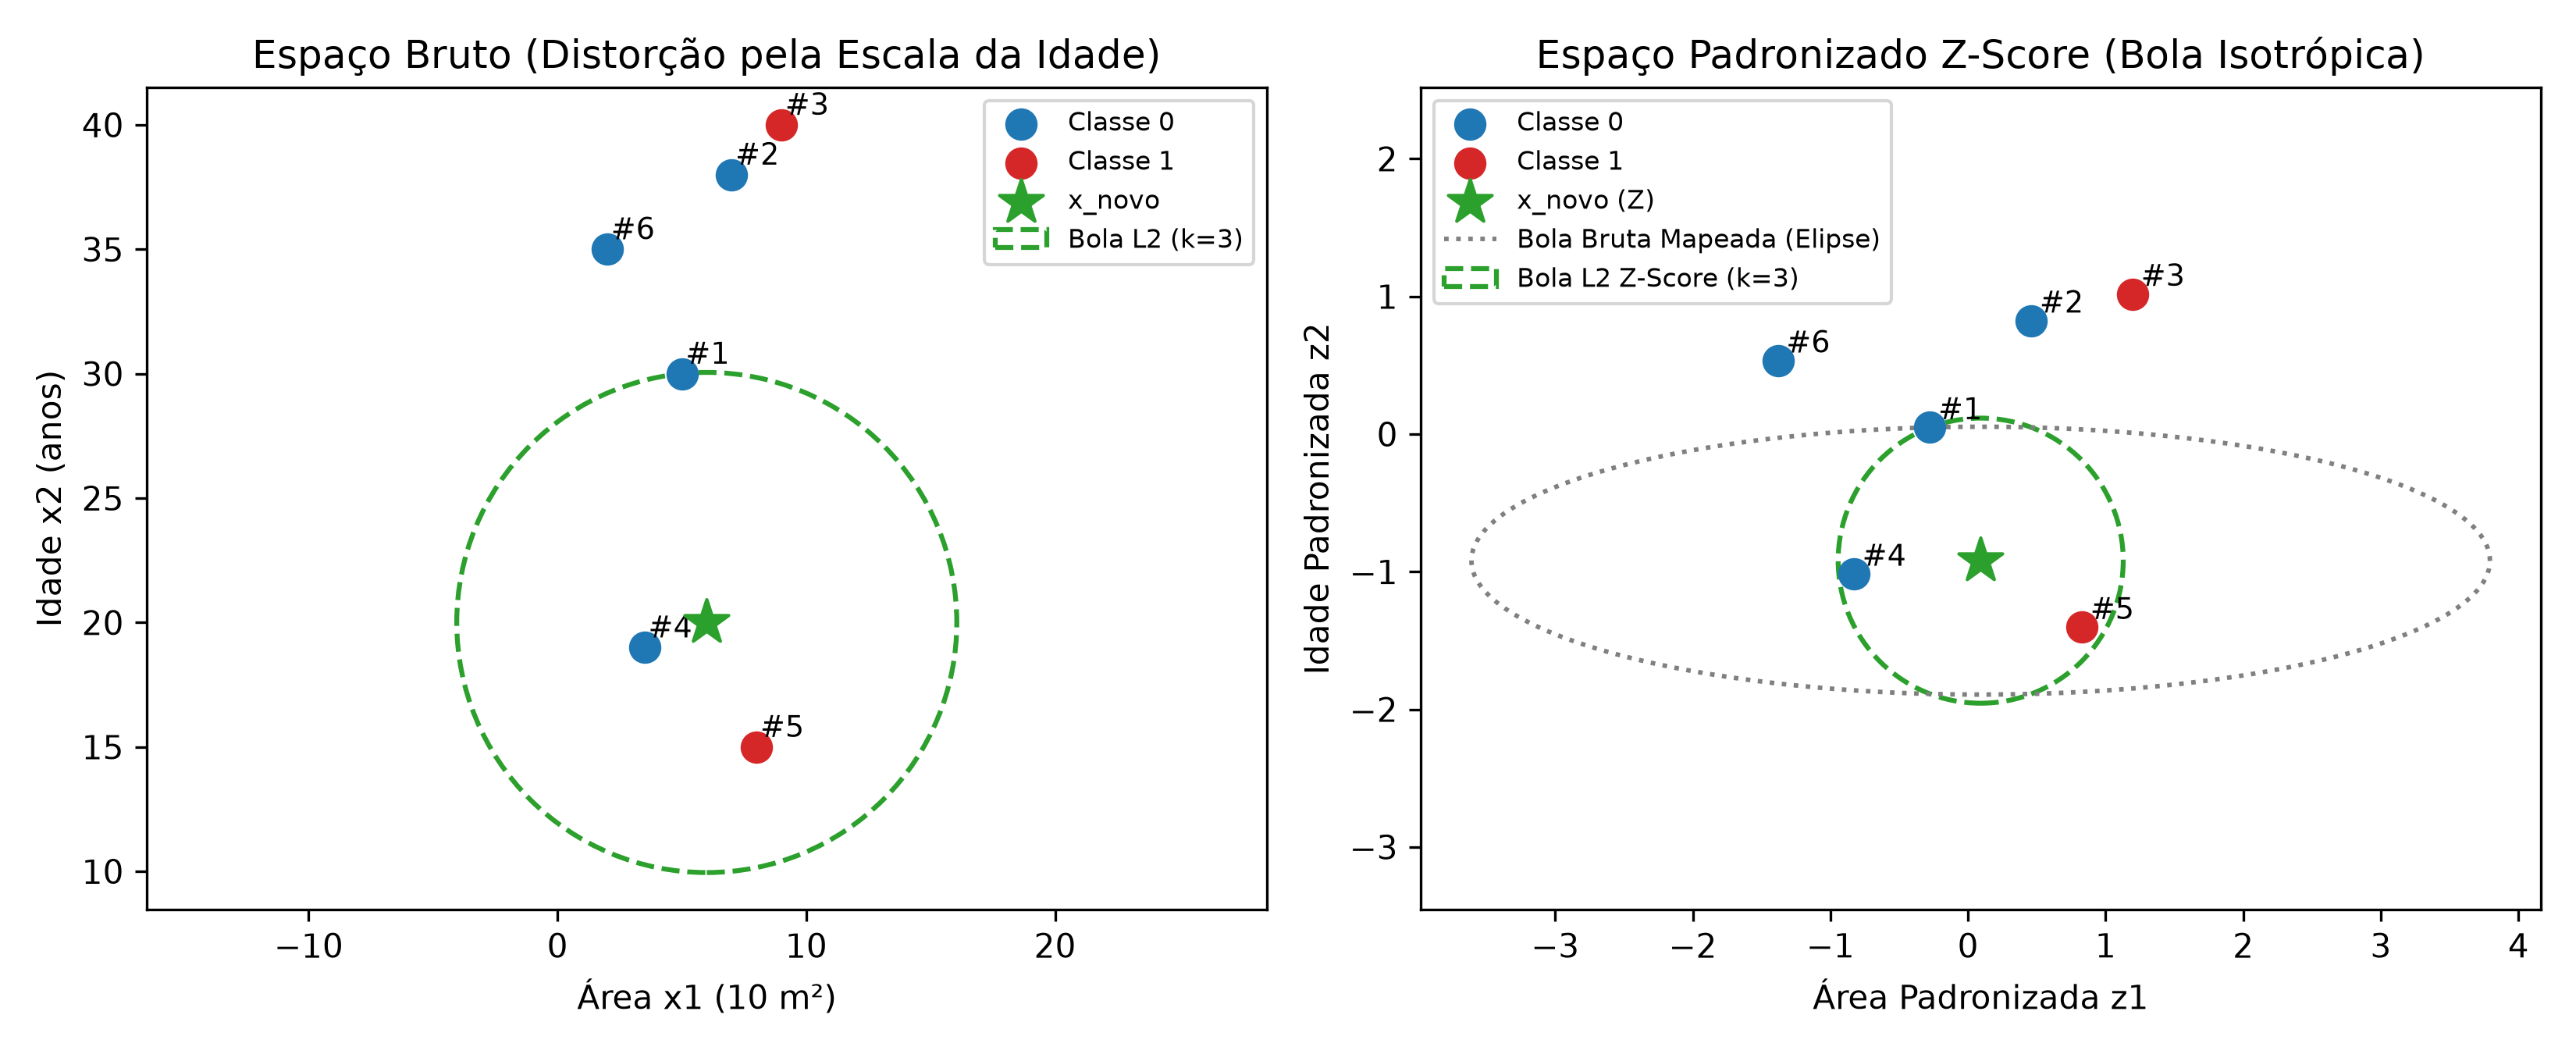
\includegraphics[width=0.92\textwidth]{../figures/q1_bolas_metricas_escala.png}
\caption{Comparação das bolas métricas $L_2$ ($k=3$) no espaço bruto e no espaço padronizado via Z-Score (com a bola bruta mapeada como elipse tracejada cinza).}
\end{figure}

% ==============================================================================
\newpage
\section{Questão 2: Regressão Linear, Posto e Mínimos Quadrados (OLS)}
% ==============================================================================

\subsection{Parte A: Formulação Matricial, Tipos de Sistemas e Posto}

\subsubsection*{A.1 e A.2. Matriz de Design, Posto e Teorema de Rouché--Capelli}
Incluindo a coluna de intercepto unitário $x_{i0} = 1$, temos:
\[
\mathbf{X} = \begin{bmatrix}
1 & 5{,}0 & 30{,}0 \\
1 & 7{,}0 & 38{,}0 \\
1 & 9{,}0 & 40{,}0 \\
1 & 3{,}5 & 19{,}0 \\
1 & 8{,}0 & 15{,}0 \\
1 & 2{,}0 & 35{,}0
\end{bmatrix} \in \mathbb{R}^{6 \times 3}, \qquad
\mathbf{y} = \begin{bmatrix} 2{,}5 \\ 3{,}8 \\ 4{,}2 \\ 1{,}9 \\ 4{,}5 \\ 1{,}2 \end{bmatrix} \in \mathbb{R}^6, \qquad
\mathbf{w} = \begin{bmatrix} w_0 \\ w_1 \\ w_2 \end{bmatrix} \in \mathbb{R}^3.
\]
O sistema $\mathbf{X}\mathbf{w} = \mathbf{y}$ é \textbf{sobredeterminado} ($N=6$ equações e $d+1=3$ incógnitas). Aplicando eliminação gaussiana na matriz aumentada $[\mathbf{X} \mid \mathbf{y}]$ ($L_i \leftarrow L_i - L_1$ para $i=2,\dots,6$, seguida de $L_3 \leftarrow L_3 - 2L_2$, etc.):
\[
\left[\begin{array}{ccc|c}
1 & 5{,}0 & 30{,}0 & 2{,}5 \\
0 & 2{,}0 & 8{,}0 & 1{,}3 \\
0 & 4{,}0 & 10{,}0 & 1{,}7 \\
0 & -1{,}5 & -11{,}0 & -0{,}6 \\
0 & 3{,}0 & -15{,}0 & 2{,}0 \\
0 & -3{,}0 & 5{,}0 & -1{,}3
\end{array}\right]
\longrightarrow
\left[\begin{array}{ccc|c}
1 & 5{,}0 & 30{,}0 & 2{,}5 \\
0 & 2{,}0 & 8{,}0 & 1{,}3 \\
0 & 0 & -6{,}0 & -0{,}9 \\
0 & 0 & 0 & 1{,}125 \\
0 & 0 & 0 & 4{,}10 \\
0 & 0 & 0 & -1{,}90
\end{array}\right].
\]
Logo, $\operatorname{rk}(\mathbf{X}) = 3$ e $\operatorname{rk}([\mathbf{X} \mid \mathbf{y}]) = 4$. Pelo \textbf{Teorema de Rouché--Capelli}, como $\operatorname{rk}(\mathbf{X}) < \operatorname{rk}([\mathbf{X} \mid \mathbf{y}])$, o sistema é \textbf{incompatível}. Geometricamente, $\mathbf{y} \notin \operatorname{Col}(\mathbf{X})$ (um subespaço de dimensão 3 em $\mathbb{R}^6$). Fisicamente, os preços reais contêm ruído de medição e fatores latentes não explicados por uma combinação linear exata de área e idade.

\subsubsection*{A.3. Multicolinearidade Exata ($x_3 = 2{,}5x_1$)}
Definindo $\tilde{\mathbf{X}} = [\mathbf{1} \quad \mathbf{x}_1 \quad \mathbf{x}_2 \quad 2{,}5\mathbf{x}_1] \in \mathbb{R}^{6 \times 4}$, a quarta coluna é combinação linear exata da segunda ($\mathbf{c}_4 = 2{,}5\mathbf{c}_2$), logo $\operatorname{Col}(\tilde{\mathbf{X}}) = \operatorname{Col}(\mathbf{X})$ e $\operatorname{rk}(\tilde{\mathbf{X}}) = \operatorname{rk}(\tilde{\mathbf{X}}^T\tilde{\mathbf{X}}) = 3 < 4$ (matriz de Gram singular). Como $\mathbf{v} = [0, -2{,}5, 0, 1]^T \in \mathcal{N}(\tilde{\mathbf{X}}) \setminus \{\mathbf{0}\}$, existem infinitos vetores de pesos ótimos $\hat{\mathbf{w}}(\alpha) = \hat{\mathbf{w}}^* + \alpha\mathbf{v}$. Entretanto, as predições $\hat{\mathbf{y}}(\alpha) = \tilde{\mathbf{X}}(\hat{\mathbf{w}}^* + \alpha\mathbf{v}) = \tilde{\mathbf{X}}\hat{\mathbf{w}}^*$ permanecem \textbf{estritamente únicas}, pois correspondem à única projeção ortogonal de $\mathbf{y}$ sobre $\operatorname{Col}(\tilde{\mathbf{X}})$.

\subsection{Parte B: Resolução por Mínimos Quadrados e Interpretação}

\subsubsection*{B.1. Matriz de Gram, Vetor $\mathbf{X}^T\mathbf{y}$ e Eliminação Gaussiana}
Calculando os produtos internos entre as colunas de $\mathbf{X}$ e $\mathbf{y}$:
\[
\mathbf{X}^T\mathbf{X} = \begin{bmatrix}
6{,}0 & 34{,}5 & 177{,}0 \\
34{,}5 & 235{,}25 & 1032{,}5 \\
177{,}0 & 1032{,}5 & 5755{,}0
\end{bmatrix}, \qquad
\mathbf{X}^T\mathbf{y} = \begin{bmatrix} 18{,}1 \\ 121{,}95 \\ 533{,}0 \end{bmatrix}.
\]
Aplicando Eliminação Gaussiana nas Equações Normais $\mathbf{X}^T\mathbf{X}\hat{\mathbf{w}} = \mathbf{X}^T\mathbf{y}$:
\begin{enumerate}
    \item $L_2 \leftarrow L_2 - 5{,}75 L_1$ e $L_3 \leftarrow L_3 - 29{,}5 L_1$:
    \[
    \left[\begin{array}{ccc|c}
    6{,}0 & 34{,}5 & 177{,}0 & 18{,}1 \\
    0 & 36{,}875 & 14{,}75 & 17{,}875 \\
    0 & 14{,}75 & 533{,}5 & -0{,}95
    \end{array}\right].
    \]
    \item $L_3 \leftarrow L_3 - \frac{14{,}75}{36{,}875}L_2 = L_3 - 0{,}4 L_2$:
    \[
    \left[\begin{array}{ccc|c}
    6{,}0 & 34{,}5 & 177{,}0 & 18{,}1 \\
    0 & 36{,}875 & 14{,}75 & 17{,}875 \\
    0 & 0 & 527{,}6 & -8{,}10
    \end{array}\right].
    \]
    \item Retrosubstituição: $\hat{w}_2 = \frac{-8{,}10}{527{,}6} \approx -0{,}01535254$, $\hat{w}_1 = \frac{17{,}875 - 14{,}75\hat{w}_2}{36{,}875} \approx 0{,}49088678$, $\hat{w}_0 = \frac{18{,}1 - 34{,}5\hat{w}_1 - 177\hat{w}_2}{6} \approx 0{,}64696761$.
\end{enumerate}

\subsubsection*{B.2. Ortogonalidade do Resíduo e Teorema de Pitágoras}
Para $\hat{\mathbf{e}} = \mathbf{y} - \mathbf{X}\hat{\mathbf{w}}$, tem-se $\mathbf{X}^T\hat{\mathbf{e}} = \mathbf{X}^T\mathbf{y} - \mathbf{X}^T\mathbf{X}\hat{\mathbf{w}} = \mathbf{0}$. Para qualquer $\mathbf{w} \in \mathbb{R}^3$, escrevendo $\mathbf{y} - \mathbf{X}\mathbf{w} = \hat{\mathbf{e}} + \mathbf{X}(\hat{\mathbf{w}} - \mathbf{w})$ e usando $\langle \hat{\mathbf{e}}, \mathbf{X}(\hat{\mathbf{w}} - \mathbf{w})\rangle = (\hat{\mathbf{w}} - \mathbf{w})^T\mathbf{X}^T\hat{\mathbf{e}} = 0$, o Teorema de Pitágoras garante:
\[
\|\mathbf{y} - \mathbf{X}\mathbf{w}\|_2^2 = \|\hat{\mathbf{e}}\|_2^2 + \|\mathbf{X}(\hat{\mathbf{w}} - \mathbf{w})\|_2^2 \ge \|\hat{\mathbf{e}}\|_2^2.
\]
Numericamente, $\|\mathbf{X}^T\hat{\mathbf{e}}\|_\infty \approx 4{,}09 \times 10^{-14} < 10^{-10}$.

\subsubsection*{B.3. Previsão para $\mathbf{x}_{\text{novo}}$ e Contraste OLS vs. $k$-NN}
$\hat{y}_{\text{lin}} = 0{,}646968 + 0{,}490887(6{,}0) - 0{,}015353(20{,}0) \approx 3{,}285237$. Enquanto o OLS ajusta um hiperplano paramétrico global ($\mathcal{O}(d)$ na inferência) que captura explicitamente a derivada parcial positiva em relação à área ($\hat{w}_1 \approx +0{,}491$), o $k$-NN faz uma média local não-paramétrica ($\mathcal{O}(Nd)$) que subestima o valor ($2{,}9667$) por incluir duas amostras vizinhas com área inferior a $60\,\text{m}^2$.

\begin{figure}[H]
\centering
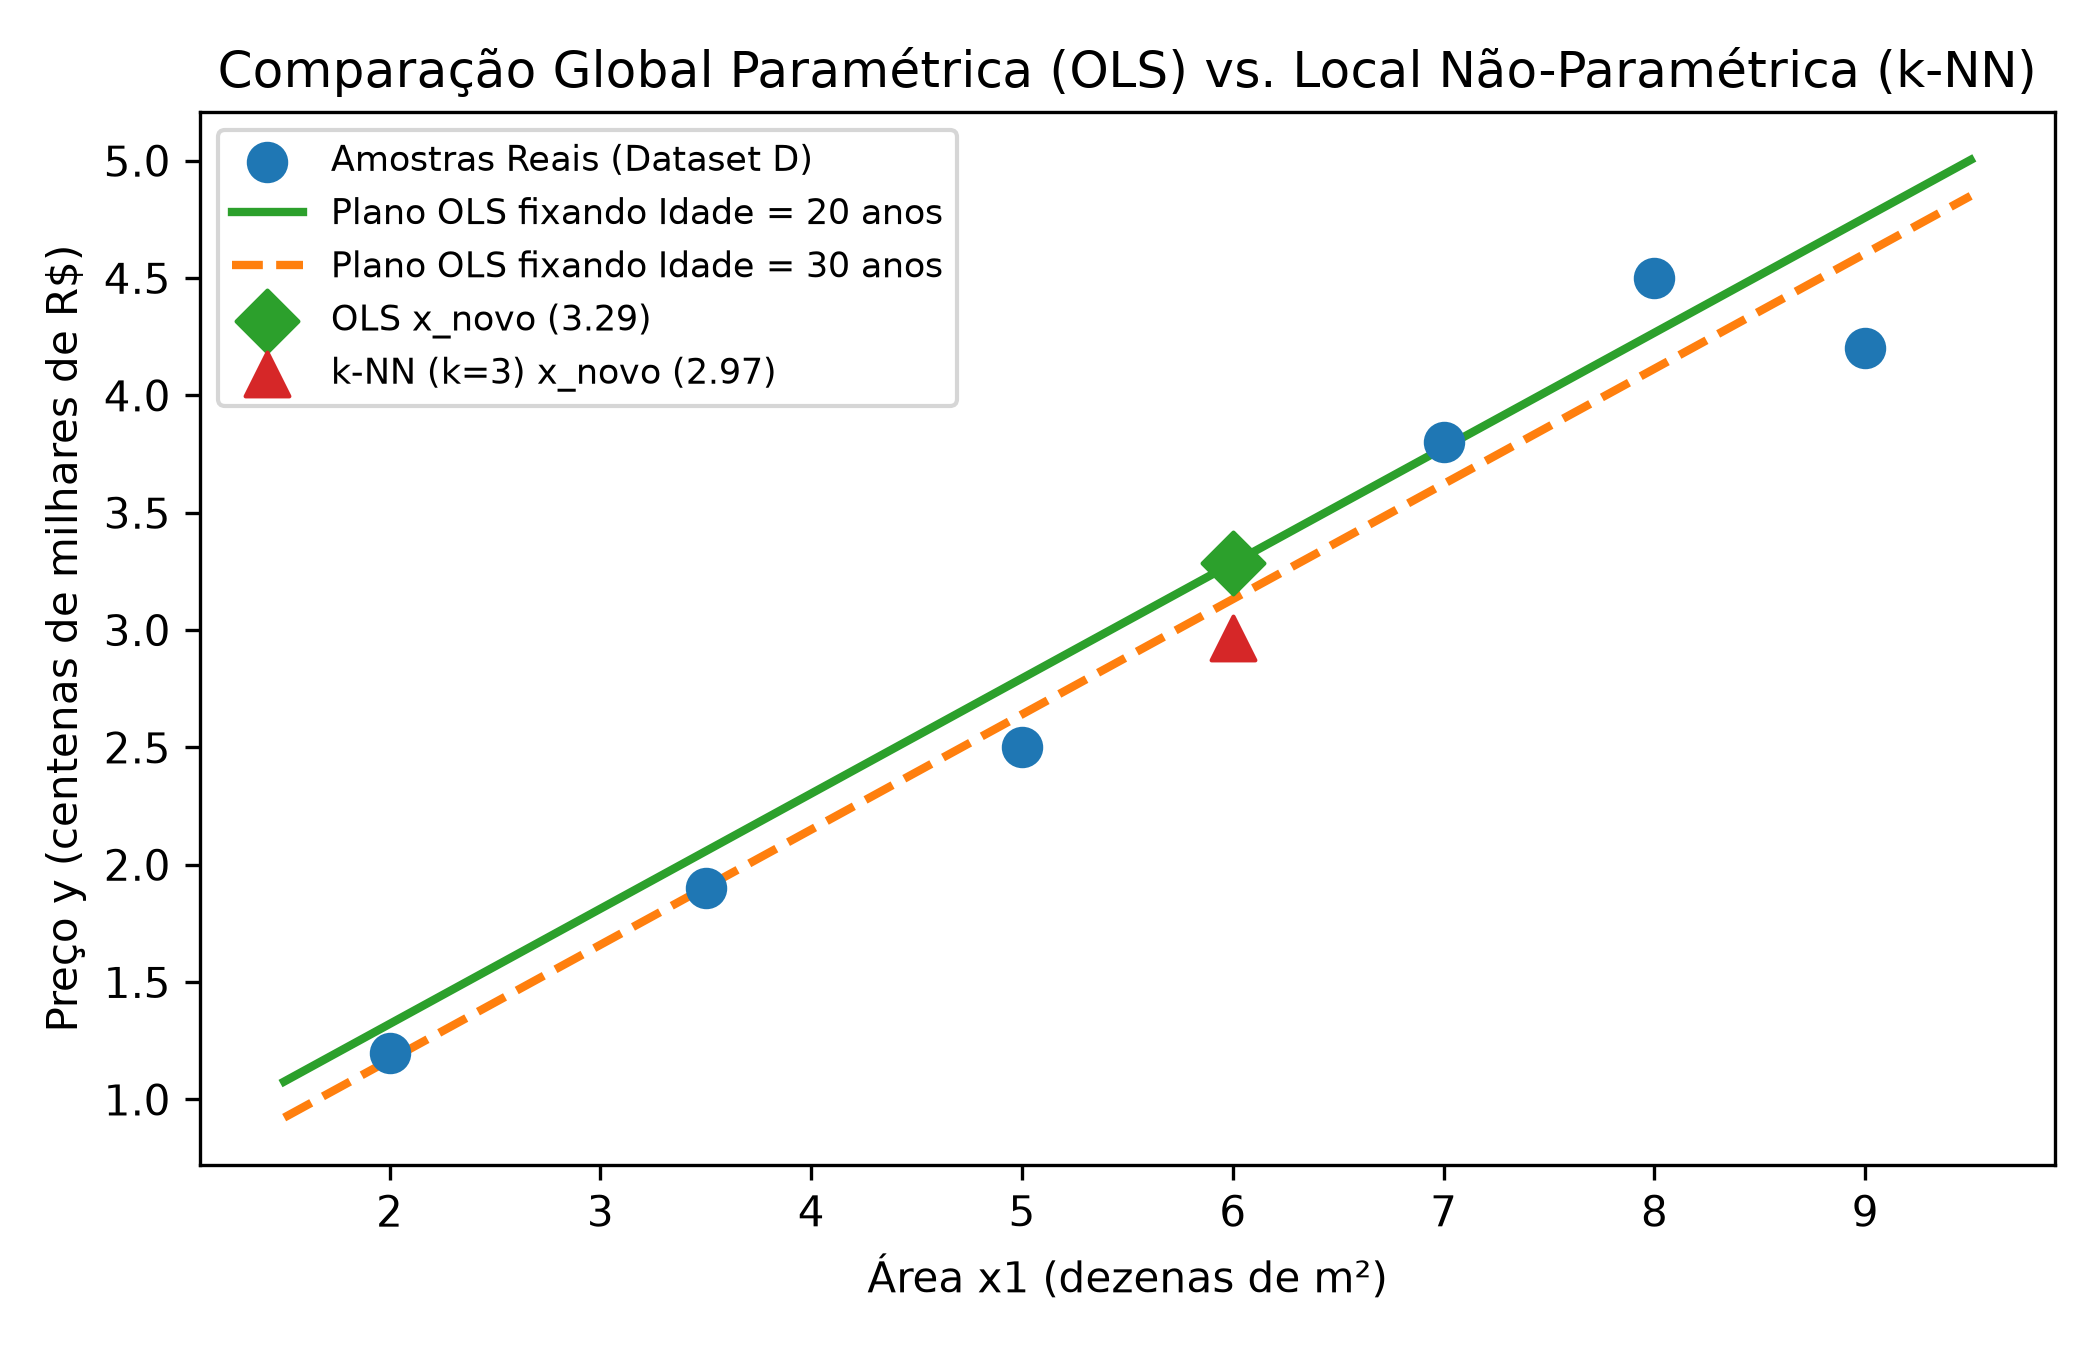
\includegraphics[width=0.78\textwidth]{../figures/q2_ols_vs_knn_superficie.png}
\caption{Comparação entre o modelo paramétrico global OLS e o estimador não-paramétrico local $k$-NN.}
\end{figure}

% ==============================================================================
\newpage
\section{Questão 3: Projeção Ortogonal, Teorema Espectral e SVD}
% ==============================================================================

\subsection{Parte A: Projeção Ortogonal e Complemento Ortogonal}
Para $\mathcal{A} = \begin{bmatrix} 1 & 1 \\ 0 & 1 \\ 1 & 0 \end{bmatrix}$ e $\mathbf{y}_{\mathcal{A}} = \begin{bmatrix} 4 \\ 1 \\ 1 \end{bmatrix}$, qualquer $\mathbf{v} = \mathcal{A}\mathbf{w} = [w_1+w_2, w_2, w_1]^T \in \operatorname{Col}(\mathcal{A})$ satisfaz $v_1 = v_2 + v_3$. Como $y_1 = 4 \ne 1 + 1 = 2$, segue que $\mathbf{y}_{\mathcal{A}} \notin \operatorname{Col}(\mathcal{A})$.
As Equações Normais $\mathcal{A}^T\mathcal{A}\hat{\mathbf{w}} = \mathcal{A}^T\mathbf{y}_{\mathcal{A}}$ são:
\[
\begin{bmatrix} 2 & 1 \\ 1 & 2 \end{bmatrix} \begin{bmatrix} \hat{w}_1 \\ \hat{w}_2 \end{bmatrix} = \begin{bmatrix} 5 \\ 5 \end{bmatrix}
\implies \hat{\mathbf{w}} = \frac{1}{3}\begin{bmatrix} 2 & -1 \\ -1 & 2 \end{bmatrix}\begin{bmatrix} 5 \\ 5 \end{bmatrix} = \begin{bmatrix} 5/3 \\ 5/3 \end{bmatrix}.
\]
Portanto, $\hat{\mathbf{y}} = \mathcal{A}\hat{\mathbf{w}} = [10/3, 5/3, 5/3]^T$ e $\hat{\mathbf{e}} = \mathbf{y}_{\mathcal{A}} - \hat{\mathbf{y}} = [2/3, -2/3, -2/3]^T$. Verifica-se $\mathcal{A}^T\hat{\mathbf{e}} = [2/3-2/3, 2/3-2/3]^T = \mathbf{0}$ e $\langle \hat{\mathbf{y}}, \hat{\mathbf{e}} \rangle = 0$, realizando a decomposição única $\mathbb{R}^3 = \operatorname{Col}(\mathcal{A}) \oplus \operatorname{Col}(\mathcal{A})^\perp$:
\[
\begin{bmatrix} 4 \\ 1 \\ 1 \end{bmatrix} = \underbrace{\begin{bmatrix} 10/3 \\ 5/3 \\ 5/3 \end{bmatrix}}_{\in \operatorname{Col}(\mathcal{A})} + \underbrace{\begin{bmatrix} 2/3 \\ -2/3 \\ -2/3 \end{bmatrix}}_{\in \operatorname{Col}(\mathcal{A})^\perp}.
\]

\subsection{Parte B: Teorema Espectral, Definitude Positiva e Condicionamento}
Para $\mathbf{S} = \mathcal{A}^T\mathcal{A} = \begin{bmatrix} 2 & 1 \\ 1 & 2 \end{bmatrix}$, o polinômio característico é $\det(\mathbf{S} - \lambda\mathbf{I}) = (2-\lambda)^2 - 1 = \lambda^2 - 4\lambda + 3 = (\lambda - 3)(\lambda - 1) = 0$, logo $\lambda_1 = 3$ e $\lambda_2 = 1$, com autovetores unitários ortogonais $\mathbf{q}_1 = \frac{1}{\sqrt{2}}[1, 1]^T$ e $\mathbf{q}_2 = \frac{1}{\sqrt{2}}[-1, 1]^T$:
\[
\mathbf{S} = \mathbf{Q}\boldsymbol{\Lambda}\mathbf{Q}^T = \frac{1}{\sqrt{2}}\begin{bmatrix} 1 & -1 \\ 1 & 1 \end{bmatrix}\begin{bmatrix} 3 & 0 \\ 0 & 1 \end{bmatrix}\frac{1}{\sqrt{2}}\begin{bmatrix} 1 & 1 \\ -1 & 1 \end{bmatrix}, \qquad \mathbf{Q}^T\mathbf{Q} = \mathbf{I}_2.
\]
Como $\mathbf{w}^T\mathbf{S}\mathbf{w} = \|\mathcal{A}\mathbf{w}\|_2^2 = (w_1+w_2)^2 + w_2^2 + w_1^2 > 0$ para todo $\mathbf{w} \ne \mathbf{0}$ (e $\lambda_1, \lambda_2 > 0$), conclui-se $\mathbf{S} \succ 0$. Os números de condição satisfazem $\kappa(\mathbf{S}) = \frac{3}{1} = 3$ e $\kappa(\mathcal{A}) = \frac{\sqrt{3}}{1} = \sqrt{3}$, provando em geral que, como $\sigma_i(\mathcal{A}) = \sqrt{\lambda_i(\mathbf{S})}$, tem-se:
\[
[\kappa(\mathcal{A})]^2 = \left(\frac{\sqrt{\lambda_{\max}(\mathbf{S})}}{\sqrt{\lambda_{\min}(\mathbf{S})}}\right)^2 = \frac{\lambda_{\max}(\mathbf{S})}{\lambda_{\min}(\mathbf{S})} = \kappa(\mathbf{S}).
\]
Em ponto flutuante IEEE 754 (\texttt{float64}, $\epsilon_{\text{máq}} \approx 2{,}22\times 10^{-16}$), formar $\mathbf{X}^T\mathbf{X}$ quadra o condicionamento ($\kappa=10^8 \to 10^{16}$), causando perda catastrófica de dígitos significativos que métodos diretos baseados em QR ou SVD evitam.

\subsection{Parte C e D: SVD Reduzida, Eckart--Young--Mirsky e Decomposição Polar}
Com $\sigma_1 = \sqrt{3}$, $\sigma_2 = 1$ e $\mathbf{V} = [\mathbf{q}_1, \mathbf{q}_2]$, os vetores singulares à esquerda $\mathbf{u}_i = \frac{1}{\sigma_i}\mathcal{A}\mathbf{v}_i$ são:
\[
\mathbf{u}_1 = \frac{1}{\sqrt{6}}\begin{bmatrix} 2 \\ 1 \\ 1 \end{bmatrix}, \qquad \mathbf{u}_2 = \frac{1}{\sqrt{2}}\begin{bmatrix} 0 \\ 1 \\ -1 \end{bmatrix}
\implies \mathcal{A} = \sigma_1\mathbf{u}_1\mathbf{v}_1^T + \sigma_2\mathbf{u}_2\mathbf{v}_2^T = \begin{bmatrix} 1 & 1 \\ 0{,}5 & 0{,}5 \\ 0{,}5 & 0{,}5 \end{bmatrix} + \begin{bmatrix} 0 & 0 \\ -0{,}5 & 0{,}5 \\ 0{,}5 & -0{,}5 \end{bmatrix}.
\]
Pelo Teorema de Eckart--Young--Mirsky, a melhor aproximação de posto 1 é $\hat{\mathcal{A}}^{(1)} = \sigma_1\mathbf{u}_1\mathbf{v}_1^T = \begin{bmatrix} 1 & 1 \\ 0{,}5 & 0{,}5 \\ 0{,}5 & 0{,}5 \end{bmatrix}$ e seu erro espectral é exatamente $\|\mathcal{A} - \hat{\mathcal{A}}^{(1)}\|_2 = \sigma_2 = 1{,}0$ (confirmado calculando $\lambda_{\max}((\mathcal{A}-\hat{\mathcal{A}}^{(1)})^T(\mathcal{A}-\hat{\mathcal{A}}^{(1)})) = 1{,}0$). Na Decomposição Polar $\mathcal{A} = \mathbf{O}\mathbf{P}$:
\[
\mathbf{O} = \mathbf{U}\mathbf{V}^T \approx \begin{bmatrix} 0{,}577350 & 0{,}577350 \\ -0{,}211325 & 0{,}788675 \\ 0{,}788675 & -0{,}211325 \end{bmatrix}, \qquad
\mathbf{P} = \mathbf{V}\boldsymbol{\Sigma}\mathbf{V}^T = \frac{1}{2}\begin{bmatrix} \sqrt{3}+1 & \sqrt{3}-1 \\ \sqrt{3}-1 & \sqrt{3}+1 \end{bmatrix} \approx \begin{bmatrix} 1{,}366025 & 0{,}366025 \\ 0{,}366025 & 1{,}366025 \end{bmatrix},
\]
onde $\mathbf{P} \succ 0$ realiza o esticamento puro nos eixos principais de $\mathbb{R}^2$ e $\mathbf{O}$ ($\mathbf{O}^T\mathbf{O}=\mathbf{I}_2$) realiza uma imersão isométrica em $\mathbb{R}^3$.

\begin{figure}[H]
\centering
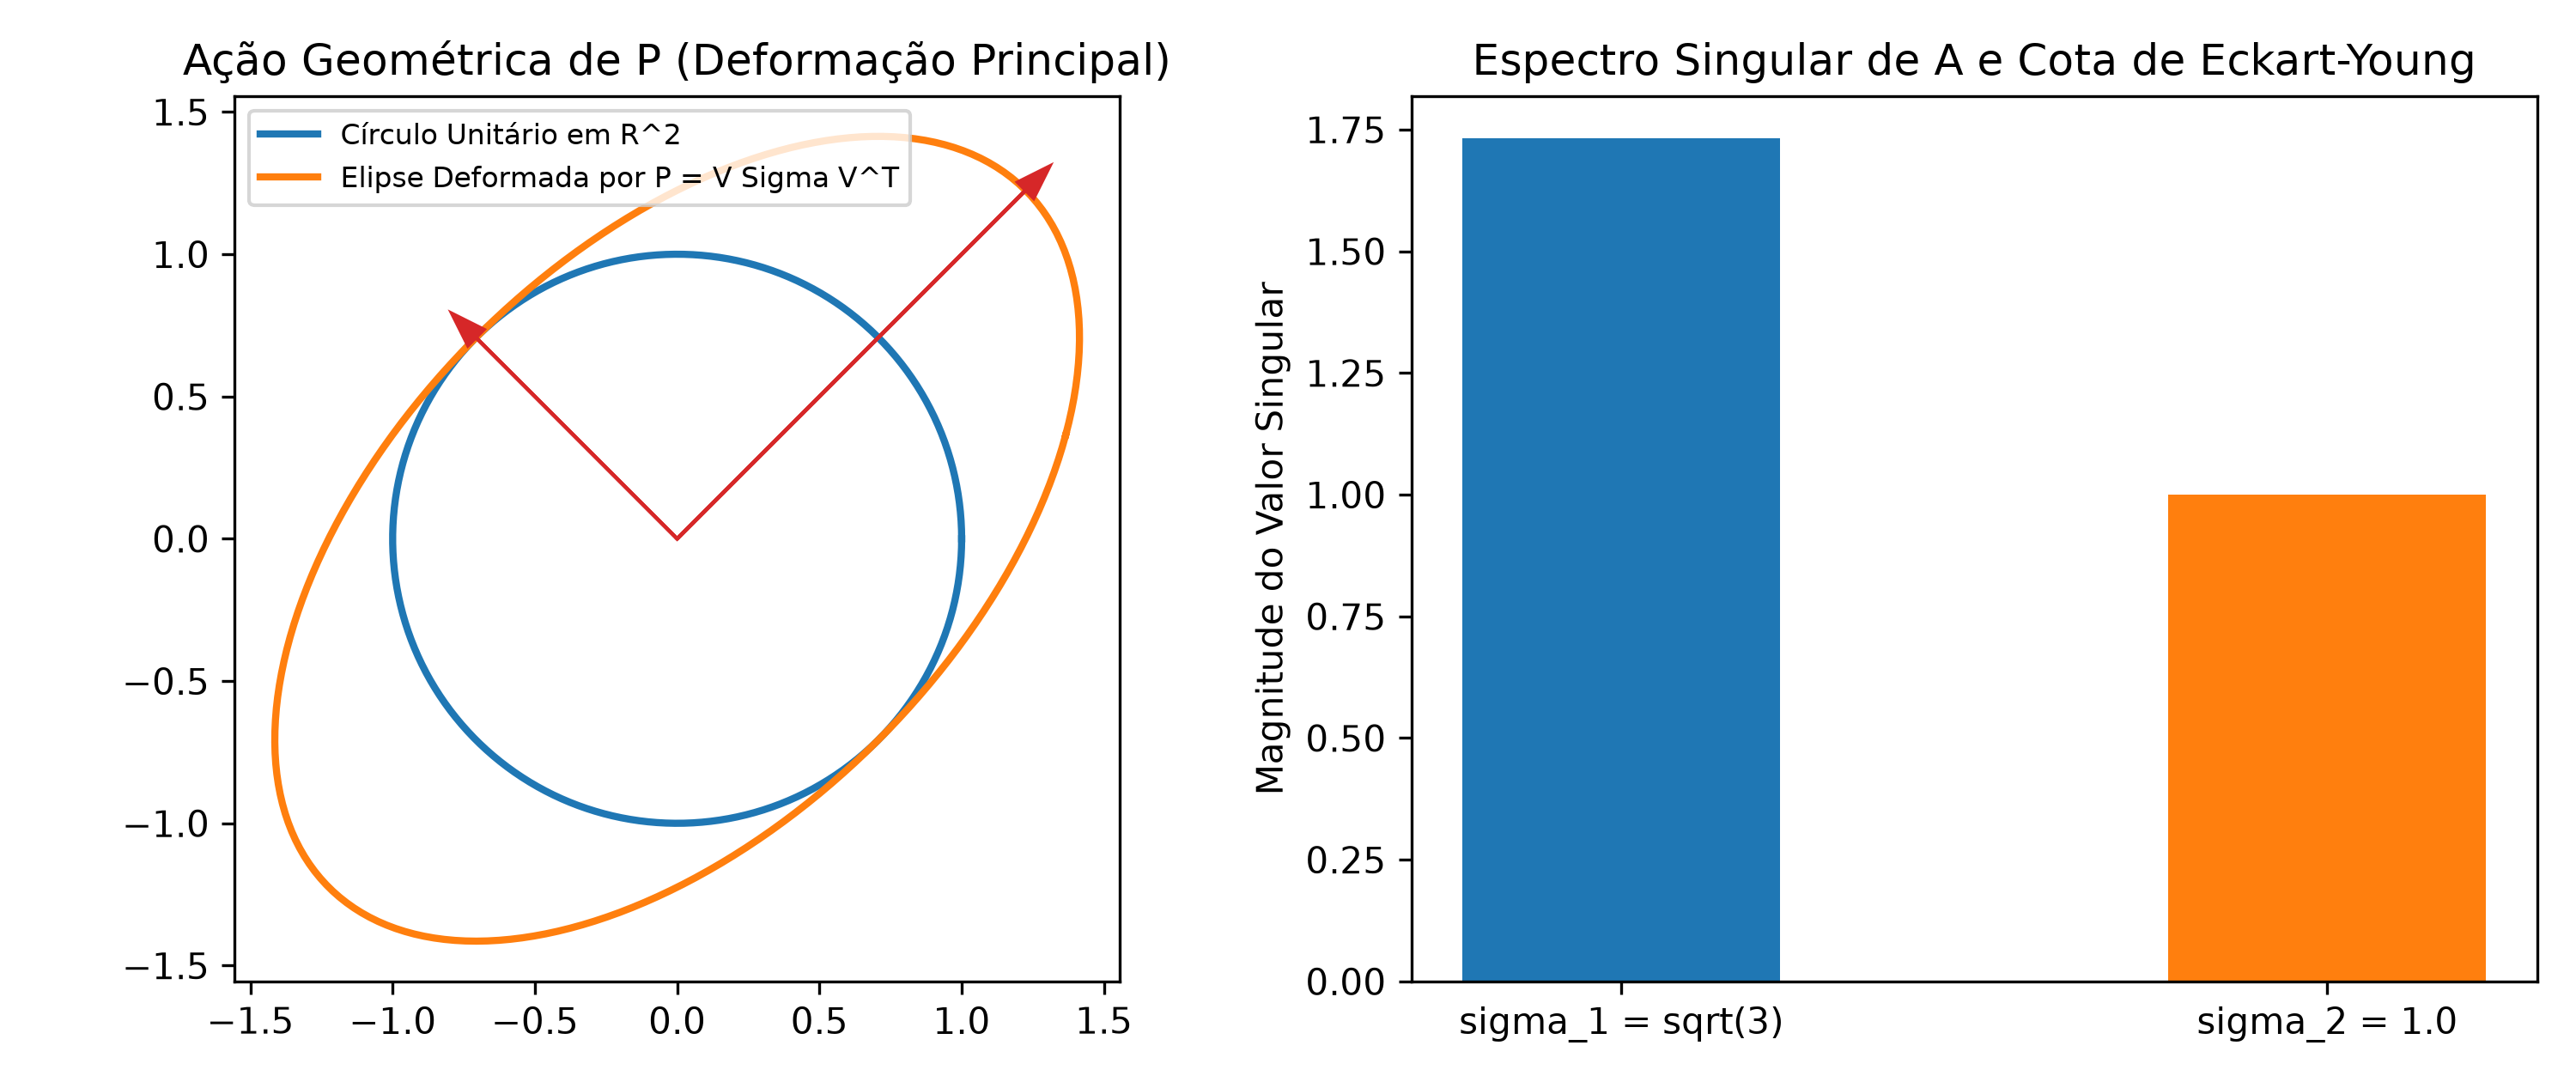
\includegraphics[width=0.90\textwidth]{../figures/q3_svd_projecao_polar.png}
\caption{Deformação principal $\mathbf{P}$ sobre o círculo unitário e espectro singular de $\mathcal{A}$.}
\end{figure}

% ==============================================================================
\newpage
\section{Questão 4: Cálculo Diferenciável, Hessiana e Vales Planos (Ridge)}
% ==============================================================================

\subsection{Parte A: Derivadas Parciais, Gradiente e Derivada Direcional}
Para $L(\boldsymbol{\beta}) = \|\mathcal{B}\boldsymbol{\beta} - \mathbf{y}_{\mathcal{B}}\|_2^2 = r_1^2 + r_2^2 + r_3^2$ com $r_1 = 2\beta_1 + \beta_2 + 3\beta_3 - 5$, $r_2 = 2\beta_2 + 2\beta_3 - 2$ e $r_3 = \beta_1 + \beta_3 - 1$:
\begin{align*}
\frac{\partial L}{\partial \beta_1} &= 2(2)r_1 + 2(0)r_2 + 2(1)r_3 = 10\beta_1 + 4\beta_2 + 14\beta_3 - 22, \\
\frac{\partial L}{\partial \beta_2} &= 2(1)r_1 + 2(2)r_2 + 2(0)r_3 = 4\beta_1 + 10\beta_2 + 14\beta_3 - 18, \\
\frac{\partial L}{\partial \beta_3} &= 2(3)r_1 + 2(2)r_2 + 2(1)r_3 = 14\beta_1 + 14\beta_2 + 28\beta_3 - 40,
\end{align*}
que se reorganizam exatamente na forma matricial $\nabla_{\boldsymbol{\beta}}L(\boldsymbol{\beta}) = 2\mathcal{B}^T\mathbf{r}(\boldsymbol{\beta}) = 2\mathcal{B}^T(\mathcal{B}\boldsymbol{\beta} - \mathbf{y}_{\mathcal{B}})$. Para $\|\mathbf{v}\|_2 = 1$ e $g(h) = L(\boldsymbol{\beta}+h\mathbf{v})$, tem-se $D_{\mathbf{v}}L(\boldsymbol{\beta}) = g'(0) = \nabla L(\boldsymbol{\beta})^T\mathbf{v}$. Pela desigualdade de Cauchy--Schwarz, $\nabla L(\boldsymbol{\beta})^T\mathbf{v} \ge -\|\nabla L(\boldsymbol{\beta})\|_2$, atingindo o mínimo em $\mathbf{v}^* = -\nabla L(\boldsymbol{\beta})/\|\nabla L(\boldsymbol{\beta})\|_2$. Em $\boldsymbol{\beta}_0 = [1, 1, 1]^T$: $\mathbf{r}(\boldsymbol{\beta}_0) = [1, 2, 1]^T$, $L(\boldsymbol{\beta}_0) = 6{,}0$, $\nabla L(\boldsymbol{\beta}_0) = [6, 10, 16]^T$, taxa de descida $-\|\nabla L(\boldsymbol{\beta}_0)\|_2 = -14\sqrt{2} \approx -19{,}7990$ e $\mathbf{u}^* = -\frac{1}{7\sqrt{2}}[3, 5, 8]^T$.

\subsection{Parte B: Jacobiano, Hessiana e Convexidade}
Sob a convenção \textit{denominator layout}, $(\mathbf{J}_{\mathbf{r}}(\boldsymbol{\beta}))_{ij} = \frac{\partial r_j}{\partial \beta_i} = \mathcal{B}_{ji} \implies \mathbf{J}_{\mathbf{r}}(\boldsymbol{\beta}) = \mathcal{B}^T$. Com $g(\mathbf{r}) = \mathbf{r}^T\mathbf{r}$ e $\nabla_{\mathbf{r}}g = 2\mathbf{r}$, a regra da cadeia vetorial $\nabla_{\boldsymbol{\beta}}L = \mathbf{J}_{\mathbf{r}}\nabla_{\mathbf{r}}g = 2\mathcal{B}^T\mathbf{r}$ corresponde exatamente ao passo reverso do algoritmo de \textit{backpropagation}. Diferenciando novamente, $\nabla^2_{\boldsymbol{\beta}} L(\boldsymbol{\beta}) = 2\mathcal{B}^T\mathcal{B}$, satisfazendo $\mathbf{v}^T(2\mathcal{B}^T\mathcal{B})\mathbf{v} = 2\|\mathcal{B}\mathbf{v}\|_2^2 \ge 0$ para todo $\mathbf{v} \in \mathbb{R}^3$ (convexidade global). Os autovalores de $2\mathcal{B}^T\mathcal{B} = \begin{bmatrix} 10 & 4 & 14 \\ 4 & 10 & 14 \\ 14 & 14 & 28 \end{bmatrix}$ são $\lambda_1 = 0$, $\lambda_2 = 6$ e $\lambda_3 = 42$; a curvatura nula $\lambda_{\min} = 0$ caracteriza um \textbf{vale plano} ao longo do núcleo $\mathcal{N}(\mathcal{B})$.

\subsection{Parte C, D e E: Vale Plano, Regularização Ridge e Diferenças Finitas}
Resolvendo $\mathcal{B}\mathbf{n} = \mathbf{0}$, obtém-se $\mathcal{N}(\mathcal{B}) = \operatorname{span}\{\mathbf{n} = [1, 1, -1]^T\}$ ($\|\mathbf{n}\|_2^2 = 3$). Para qualquer $\boldsymbol{\beta}(t) = \boldsymbol{\beta}^* + t\mathbf{n}$, como $\mathcal{B}\mathbf{n} = \mathbf{0}$, segue $\nabla L(\boldsymbol{\beta}(t)) = \mathbf{0}$ e $L(\boldsymbol{\beta}(t)) = L(\boldsymbol{\beta}^*) = 16/21 \approx 0{,}761905$.
Na regularização Ridge $L_\lambda(\boldsymbol{\beta}) = \|\mathcal{B}\boldsymbol{\beta}-\mathbf{y}_{\mathcal{B}}\|_2^2 + \lambda\|\boldsymbol{\beta}\|_2^2$:
\[
\nabla_{\boldsymbol{\beta}}L_\lambda(\boldsymbol{\beta}) = 2\left[(\mathcal{B}^T\mathcal{B} + \lambda\mathbf{I})\boldsymbol{\beta} - \mathcal{B}^T\mathbf{y}_{\mathcal{B}}\right], \qquad
\nabla^2_{\boldsymbol{\beta}}L_\lambda(\boldsymbol{\beta}) = 2(\mathcal{B}^T\mathcal{B} + \lambda\mathbf{I}).
\]
Pelo Teorema Espectral ($2\mathcal{B}^T\mathcal{B} = \mathbf{Q}\boldsymbol{\Lambda}\mathbf{Q}^T$), os autovalores deslocam-se para $\mu_i = \lambda_i + 2\lambda \ge 2\lambda > 0$ (para $\lambda=1$: $\{2, 8, 44\}$), garantindo estrita convexidade e único minimizador $\boldsymbol{\beta}_1 = (\mathcal{B}^T\mathcal{B}+\mathbf{I})^{-1}\mathcal{B}^T\mathbf{y}_{\mathcal{B}} = [31/44, 9/44, 10/11]^T$. A segunda derivada direcional (curvatura) ao longo de $\mathbf{n}$ torna-se $\mathbf{n}^T\nabla^2 L_\lambda \mathbf{n} = 2\lambda\|\mathbf{n}\|_2^2 = 6$ (de modo que $L_\lambda(\boldsymbol{\beta}_\lambda + t\mathbf{n}) - L_\lambda(\boldsymbol{\beta}_\lambda) = \lambda\|\mathbf{n}\|_2^2 t^2 = 3t^2$).

Na diferença finita central $\frac{L(\boldsymbol{\beta}+h\mathbf{e}_j)-L(\boldsymbol{\beta}-h\mathbf{e}_j)}{2h} = \frac{\partial L}{\partial \beta_j} + \frac{h^2}{6}\frac{\partial^3 L}{\partial \beta_j^3} + \mathcal{O}(h^4)$, como $L$ é um polinômio quadrático, todas as derivadas de ordem $\ge 3$ são identicamente nulas, tornando o erro de truncamento $\mathcal{O}(h^2)$ nulo; a discrepância observada ($\approx 1{,}05 \times 10^{-10}$ para $h=10^{-5}$) advém exclusivamente do cancelamento catastrófico de ponto flutuante $\mathcal{O}(\epsilon_{\text{máq}}/h)$.

\begin{figure}[H]
\centering
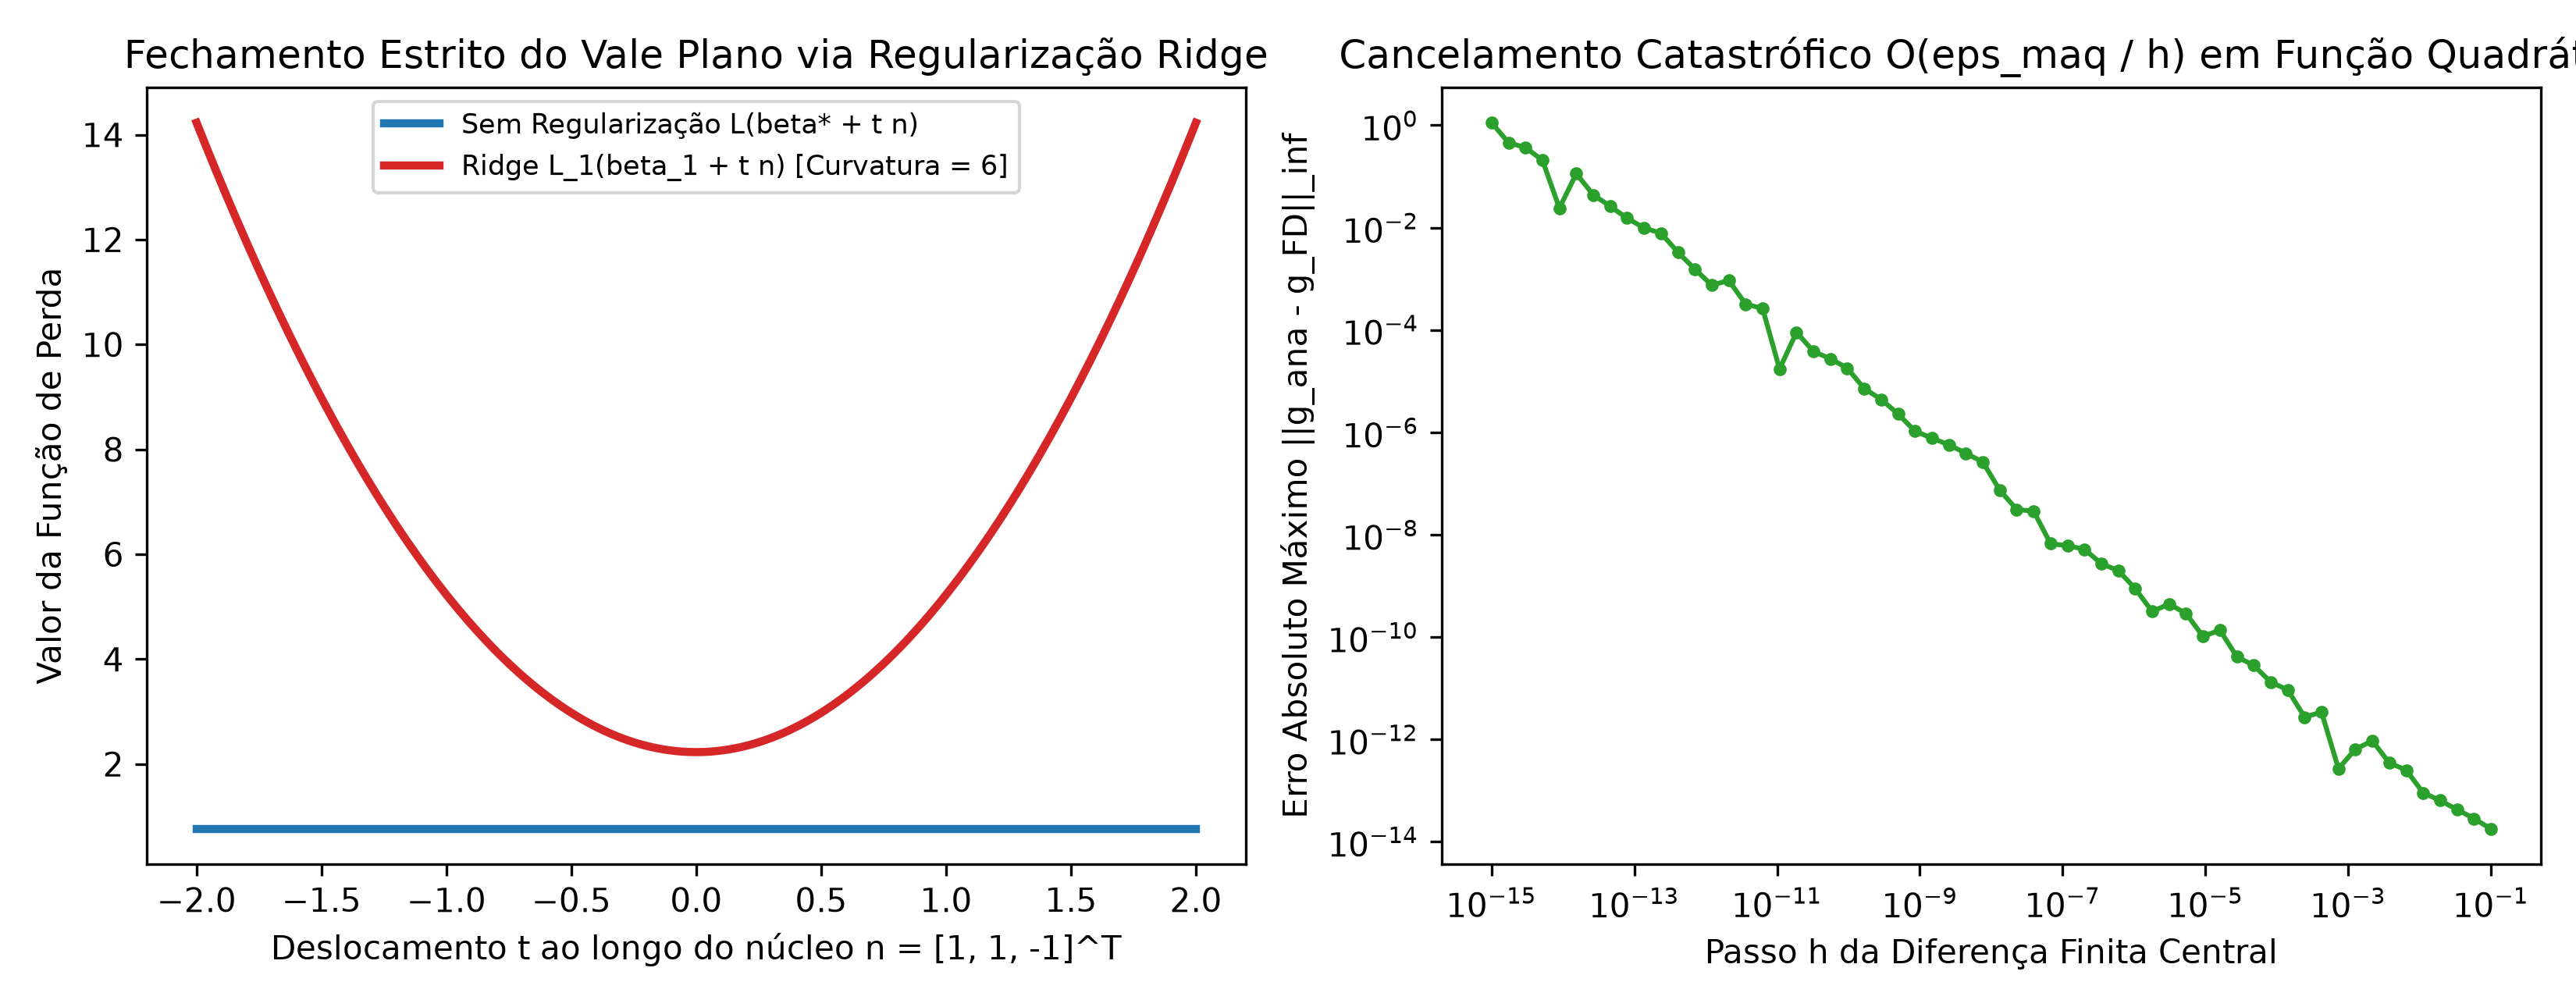
\includegraphics[width=0.92\textwidth]{../figures/q4_vale_plano_vs_ridge.png}
\caption{Fechamento do vale plano via Ridge e cancelamento catastrófico $\mathcal{O}(\epsilon_{\text{máq}}/h)$ na diferença finita central.}
\end{figure}

% ==============================================================================
\newpage
\section{Questão 5: Convergência de 1ª Ordem e Regressão Logística}
% ==============================================================================

\subsection{Parte A: Direção de Maior Descida, $L$-Suavidade e Lema da Descida}
Pela desigualdade de Cauchy--Schwarz, $D_{\mathbf{u}}f(\mathbf{w}) = \nabla f(\mathbf{w})^T\mathbf{u} \ge -\|\nabla f(\mathbf{w})\|_2$ ($\|\mathbf{u}\|_2=1$), com mínimo em $\mathbf{u}^* = -\nabla f(\mathbf{w})/\|\nabla f(\mathbf{w})\|_2$, justificando $\mathbf{w}_{k+1} = \mathbf{w}_k - \alpha\nabla f(\mathbf{w}_k)$. Uma função $f \in C^2(\mathbb{R}^d)$ é $L$-suave ($\|\nabla f(\mathbf{y})-\nabla f(\mathbf{x})\|_2 \le L\|\mathbf{y}-\mathbf{x}\|_2$) se e somente se $\lambda_{\max}(\nabla^2 f(\mathbf{w})) \le L$ para todo $\mathbf{w}$. Aplicando o Teorema Fundamental do Cálculo a $g(t) = f(\mathbf{x} + t(\mathbf{y}-\mathbf{x}))$:
\[
f(\mathbf{y}) - f(\mathbf{x}) - \nabla f(\mathbf{x})^T(\mathbf{y}-\mathbf{x}) = \int_0^1 [\nabla f(\mathbf{x}+t(\mathbf{y}-\mathbf{x}))-\nabla f(\mathbf{x})]^T(\mathbf{y}-\mathbf{x})\,dt \le \int_0^1 L t \|\mathbf{y}-\mathbf{x}\|_2^2\,dt = \frac{L}{2}\|\mathbf{y}-\mathbf{x}\|_2^2.
\]
Substituindo $\mathbf{y} = \mathbf{w}_{k+1} = \mathbf{w}_k - \alpha\nabla f(\mathbf{w}_k)$, obtém-se $f(\mathbf{w}_{k+1}) \le f(\mathbf{w}_k) - \alpha\left(1 - \frac{L\alpha}{2}\right)\|\nabla f(\mathbf{w}_k)\|_2^2$, garantindo decréscimo estrito para $0 < \alpha < \frac{2}{L}$ e redução ótima de $\frac{1}{2L}\|\nabla f(\mathbf{w}_k)\|_2^2$ em $\alpha^* = \frac{1}{L}$.

\subsection{Parte B: Dinâmica Espectral do Erro e Contração de Chebyshev}
Para $f(\mathbf{w}) = \frac{1}{2}\mathbf{w}^T\mathbf{A}\mathbf{w} - \mathbf{b}^T\mathbf{w}$ ($\mathbf{A} \succ 0, \mathbf{A}\mathbf{w}^*=\mathbf{b}$), temos $\nabla f(\mathbf{w}_k) = \mathbf{A}\mathbf{e}_k$ e $\mathbf{e}_{k+1} = (\mathbf{I}-\alpha\mathbf{A})\mathbf{e}_k$. Na base modal $\tilde{\mathbf{e}}_k = \mathbf{Q}^T\mathbf{e}_k$ ($\mathbf{A}=\mathbf{Q}\boldsymbol{\Lambda}\mathbf{Q}^T$), as componentes desacoplam-se em $\tilde{e}_{k+1,i} = (1-\alpha\lambda_i)\tilde{e}_{k,i}$. Resolvendo o minimax $\min_{\alpha>0}\max\{1-\alpha\lambda_{\min}, \alpha\lambda_{\max}-1\}$ na interseção $1-\alpha^*\lambda_{\min} = \alpha^*\lambda_{\max}-1$, obtemos:
\[
\alpha^* = \frac{2}{\lambda_{\max} + \lambda_{\min}}, \qquad \rho^* = \frac{\lambda_{\max}-\lambda_{\min}}{\lambda_{\max}+\lambda_{\min}} = \frac{\kappa-1}{\kappa+1}.
\]
Consequentemente, $f(\mathbf{w}_k) - f^* = \frac{1}{2}\sum_{i=1}^d \lambda_i (1-\alpha^*\lambda_i)^{2k}\tilde{e}_{0,i}^2 \le (\rho^*)^{2k}\left(\frac{1}{2}\sum_{i=1}^d \lambda_i\tilde{e}_{0,i}^2\right) = (\rho^*)^{2k}(f(\mathbf{w}_0) - f^*)$.

\subsection{Parte C: Mau Condicionamento e Pré-Condicionamento Z-Score}
Para $\kappa \gg 1$, as curvas de nível são elipsoides estreitos e o gradiente $-\nabla f(\mathbf{w})$ aponta quase perpendicularmente ao fundo do vale, causando ziguezague transversal com $1 - \alpha^*\lambda_{\max} = -\rho^* \approx -1$. Sob $\tilde{\mathbf{X}}_c = \mathbf{X}_c\mathbf{D}^{-1/2}$ ($\mathbf{D} = \operatorname{diag}(s_1^2,\dots,s_d^2)$), a Hessiana média transforma-se na matriz de correlação de Pearson $\tilde{\mathbf{H}} = \mathbf{D}^{-1/2}\mathbf{H}\mathbf{D}^{-1/2}$ ($\tilde{H}_{jj}=1$). No Dataset $\mathcal{D}$ (com coluna de \textit{bias}), o condicionamento reduz-se de $\kappa(2\mathbf{X}^T\mathbf{X}) = 14\,714{,}2235$ para $1{,}3410$ (\texttt{ddof=1}) ou $1{,}2350$ (\texttt{ddof=0}). Sob $\tilde{\mathbf{w}} = \mathbf{D}^{1/2}\mathbf{w}$, a GD em $\tilde{\mathbf{X}}$ equivale exatamente ao Gradiente Pré-Condicionado de Jacobi $\mathbf{w}_{k+1} = \mathbf{w}_k - \alpha\mathbf{D}^{-1}\nabla f(\mathbf{w}_k)$.

\subsection{Parte D: Regressão Logística Regularizada ($\lambda = 0{,}1$)}
Para $\mathcal{L}(\mathbf{w}) = -\frac{1}{N}\sum_{n=1}^N [c_n\ln\hat{y}_n + (1-c_n)\ln(1-\hat{y}_n)] + \lambda\|\mathbf{w}\|_2^2$ com $\hat{y}_n = \sigma(\mathbf{w}^T\mathbf{x}_n)$ e $\sigma'(z) = \sigma(z)(1-\sigma(z))$:
\[
\nabla_{\mathbf{w}}\mathcal{L}(\mathbf{w}) = \frac{1}{N}\mathbf{X}^T(\hat{\mathbf{y}} - \mathbf{c}) + 2\lambda\mathbf{w}, \qquad
\nabla^2_{\mathbf{w}}\mathcal{L}(\mathbf{w}) = \frac{1}{N}\mathbf{X}^T\mathbf{S}\mathbf{X} + 2\lambda\mathbf{I}, \quad \mathbf{S}=\operatorname{diag}(\hat{y}_n(1-\hat{y}_n)).
\]
Como $\nabla\mathcal{L}(\mathbf{w}) = \mathbf{0}$ acopla exponenciais não-lineares com termos lineares, trata-se de um sistema transcendental sem solução fechada. Como $\hat{y}_n(1-\hat{y}_n) > 0$, $\mathbf{S} \succ 0$ e $\nabla^2\mathcal{L}(\mathbf{w}) \succeq 2\lambda\mathbf{I} \succ 0$, provando $2\lambda$-convexidade forte global e unicidade de $\mathbf{w}^*$. Como as classes de $\mathcal{D}$ são linearmente separáveis, $\lambda > 0$ é indispensável para evitar $\|\mathbf{w}_k\|_2 \to \infty$. Após 2000 iterações nos dados padronizados (\texttt{ddof=1}), obtém-se $\hat{\mathbf{w}} = [-0{,}407885, 0{,}896095, -0{,}221284]^T$, probabilidades $[0{,}3394, 0{,}4557, 0{,}6082, 0{,}2839, 0{,}6559, 0{,}1464]^T$ e acurácia de treino de $100{,}0\%$ ($6/6$).

\begin{figure}[H]
\centering
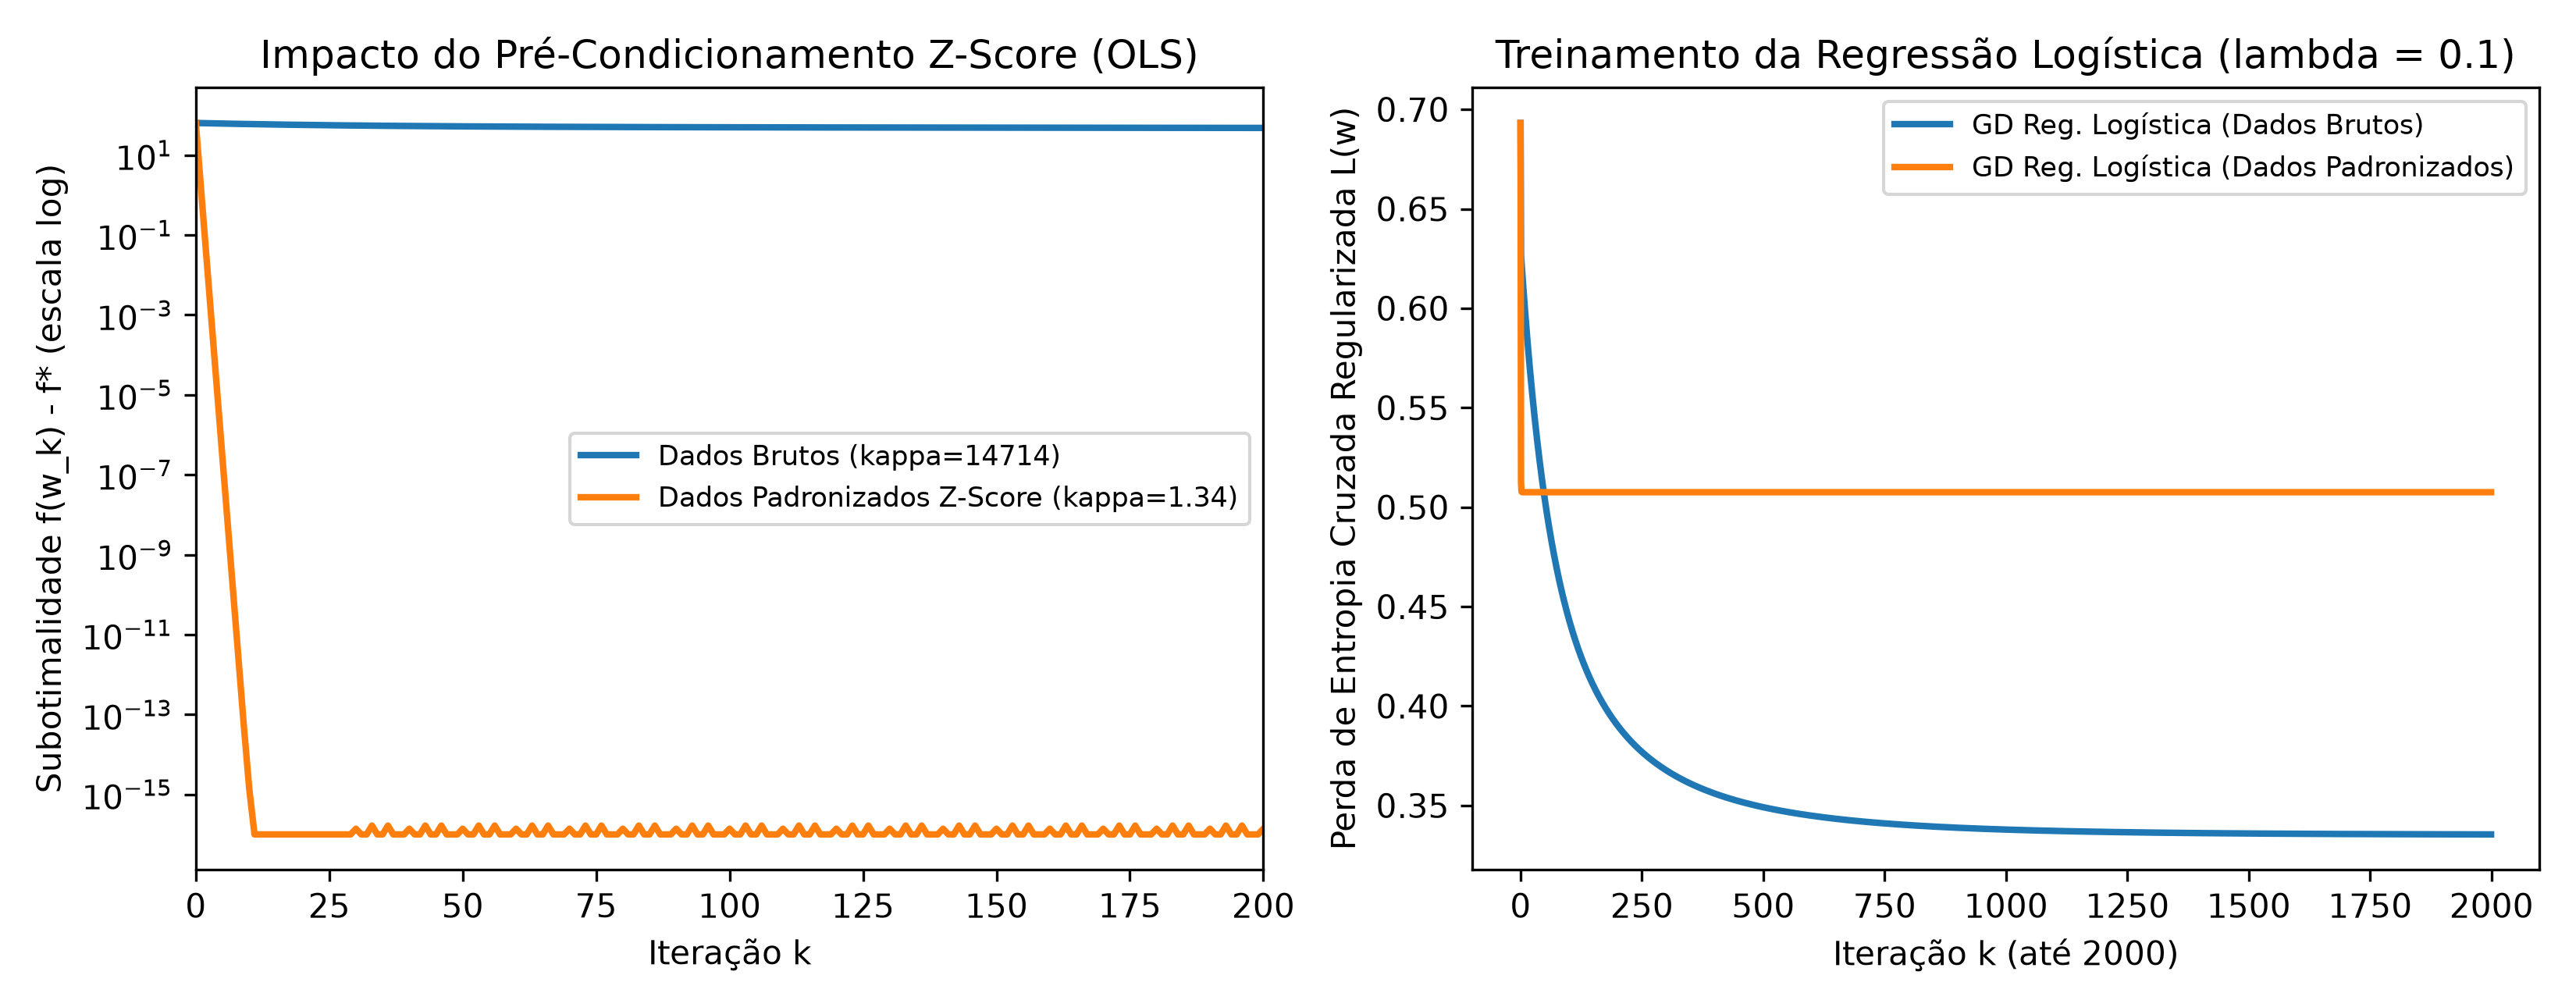
\includegraphics[width=0.92\textwidth]{../figures/q5_condicionamento_gd_logistica.png}
\caption{Impacto do pré-condicionamento Z-Score no OLS e convergência da Regressão Logística ($\lambda=0{,}1$).}
\end{figure}

% ==============================================================================
\newpage
\section{Questão 6: Otimização Estocástica, Momento, Adam e Newton}
% ==============================================================================

\subsection{Parte A e B: Estimador Mini-Batch e Condições de Robbins--Monro}
Sob amostragem uniforme com reposição ($|B|=B$), pela linearidade da esperança e independência entre amostras do lote:
\[
\mathbb{E}_B[g_B(\mathbf{w})] = \frac{1}{B}\sum_{k=1}^B \mathbb{E}_{i_k}[\nabla\ell_{i_k}(\mathbf{w})] = \nabla\mathcal{L}(\mathbf{w}), \qquad
\operatorname{Var}(g_B(\mathbf{w})) = \frac{1}{B^2}\sum_{k=1}^B \operatorname{Var}(\nabla\ell_{i_k}(\mathbf{w})) = \frac{\sigma^2}{B}.
\]
As condições de Robbins--Monro exigem $\sum_{t=1}^\infty \alpha_t = \infty$ (para que o algoritmo alcance $\mathbf{w}^*$ a qualquer distância finita de $\mathbf{w}_0$) e $\sum_{t=1}^\infty \alpha_t^2 < \infty$ (para dissipar a variância acumulada do ruído estocástico). Para $\alpha_t = \alpha_0 / t^\gamma$, pelo critério da $p$-série, exige-se $\gamma \le 1$ e $2\gamma > 1 \implies \gamma \in (1/2, 1]$.

\subsection{Parte C e D: Polyak, Nesterov (NAG), RMSProp e Adam}
No algoritmo de Polyak ($\mathbf{v}_{t+1} = \beta\mathbf{v}_t + \alpha\nabla f(\mathbf{w}_t)$), $\mathbf{v}_t = \alpha\sum_{k=0}^{t-1}\beta^k\nabla f(\mathbf{w}_{t-1-k})$ amortiza oscilações transversais alternadas e acumula ganho de até $\frac{1}{1-\beta}$ na direção longitudinal (equivalente a uma esfera com inércia sob atrito viscoso). O NAG avalia o gradiente no ponto antecipado $\mathbf{w}_t - \beta\mathbf{v}_t$, introduzindo um freio preditivo de segunda ordem que evita \textit{overshooting}. No RMSProp, $\mathbf{v}_t = \beta_2\mathbf{v}_{t-1} + (1-\beta_2)\mathbf{g}_t\odot\mathbf{g}_t$ atua como pré-condicionador diagonal empírico $\hat{\mathbf{D}}_t = \operatorname{diag}(\sqrt{\mathbf{v}_t}+\epsilon)$. No Adam, expandindo $\mathbf{m}_t = (1-\beta_1)\sum_{i=1}^t \beta_1^{t-i}\mathbf{g}_i$ a partir de $\mathbf{m}_0=\mathbf{0}$, obtém-se $\mathbb{E}[\mathbf{m}_t] = \mathbb{E}[\mathbf{g}_t](1-\beta_1^t)$, justificando os estimadores corrigidos $\hat{\mathbf{m}}_t = \mathbf{m}_t/(1-\beta_1^t)$ e $\hat{\mathbf{v}}_t = \mathbf{v}_t/(1-\beta_2^t)$.

\subsection{Parte E: Validação Numérica e Método de Newton em 1 Iteração}
Para $f(w_1, w_2) = \frac{1}{2}(100w_1^2 + w_2^2)$ ($\kappa=100$), partindo de $\mathbf{w}_0 = [10, 10]^T$ até $\|\mathbf{w}_t\|_2 < 10^{-6}$: GD Chebyshev ($824$ iterações), Polyak ($302$), NAG ($209$), Adam ($353$) e Método de Newton Exato ($1$ iteração). Para qualquer quadrática $f(\mathbf{w}) = \frac{1}{2}\mathbf{w}^T\mathbf{A}\mathbf{w} - \mathbf{b}^T\mathbf{w} + c$ ($\mathbf{A} \succ 0, \mathbf{w}^*=\mathbf{A}^{-1}\mathbf{b}$), um único passo de Newton fornece:
\[
\mathbf{w}_1 = \mathbf{w}_0 - [\nabla^2 f(\mathbf{w}_0)]^{-1}\nabla f(\mathbf{w}_0) = \mathbf{w}_0 - \mathbf{A}^{-1}(\mathbf{A}\mathbf{w}_0 - \mathbf{b}) = \mathbf{A}^{-1}\mathbf{b} = \mathbf{w}^*,
\]
atingindo o mínimo global exato em 1 única iteração, independentemente de $\kappa(\mathbf{A})$.

\begin{figure}[H]
\centering
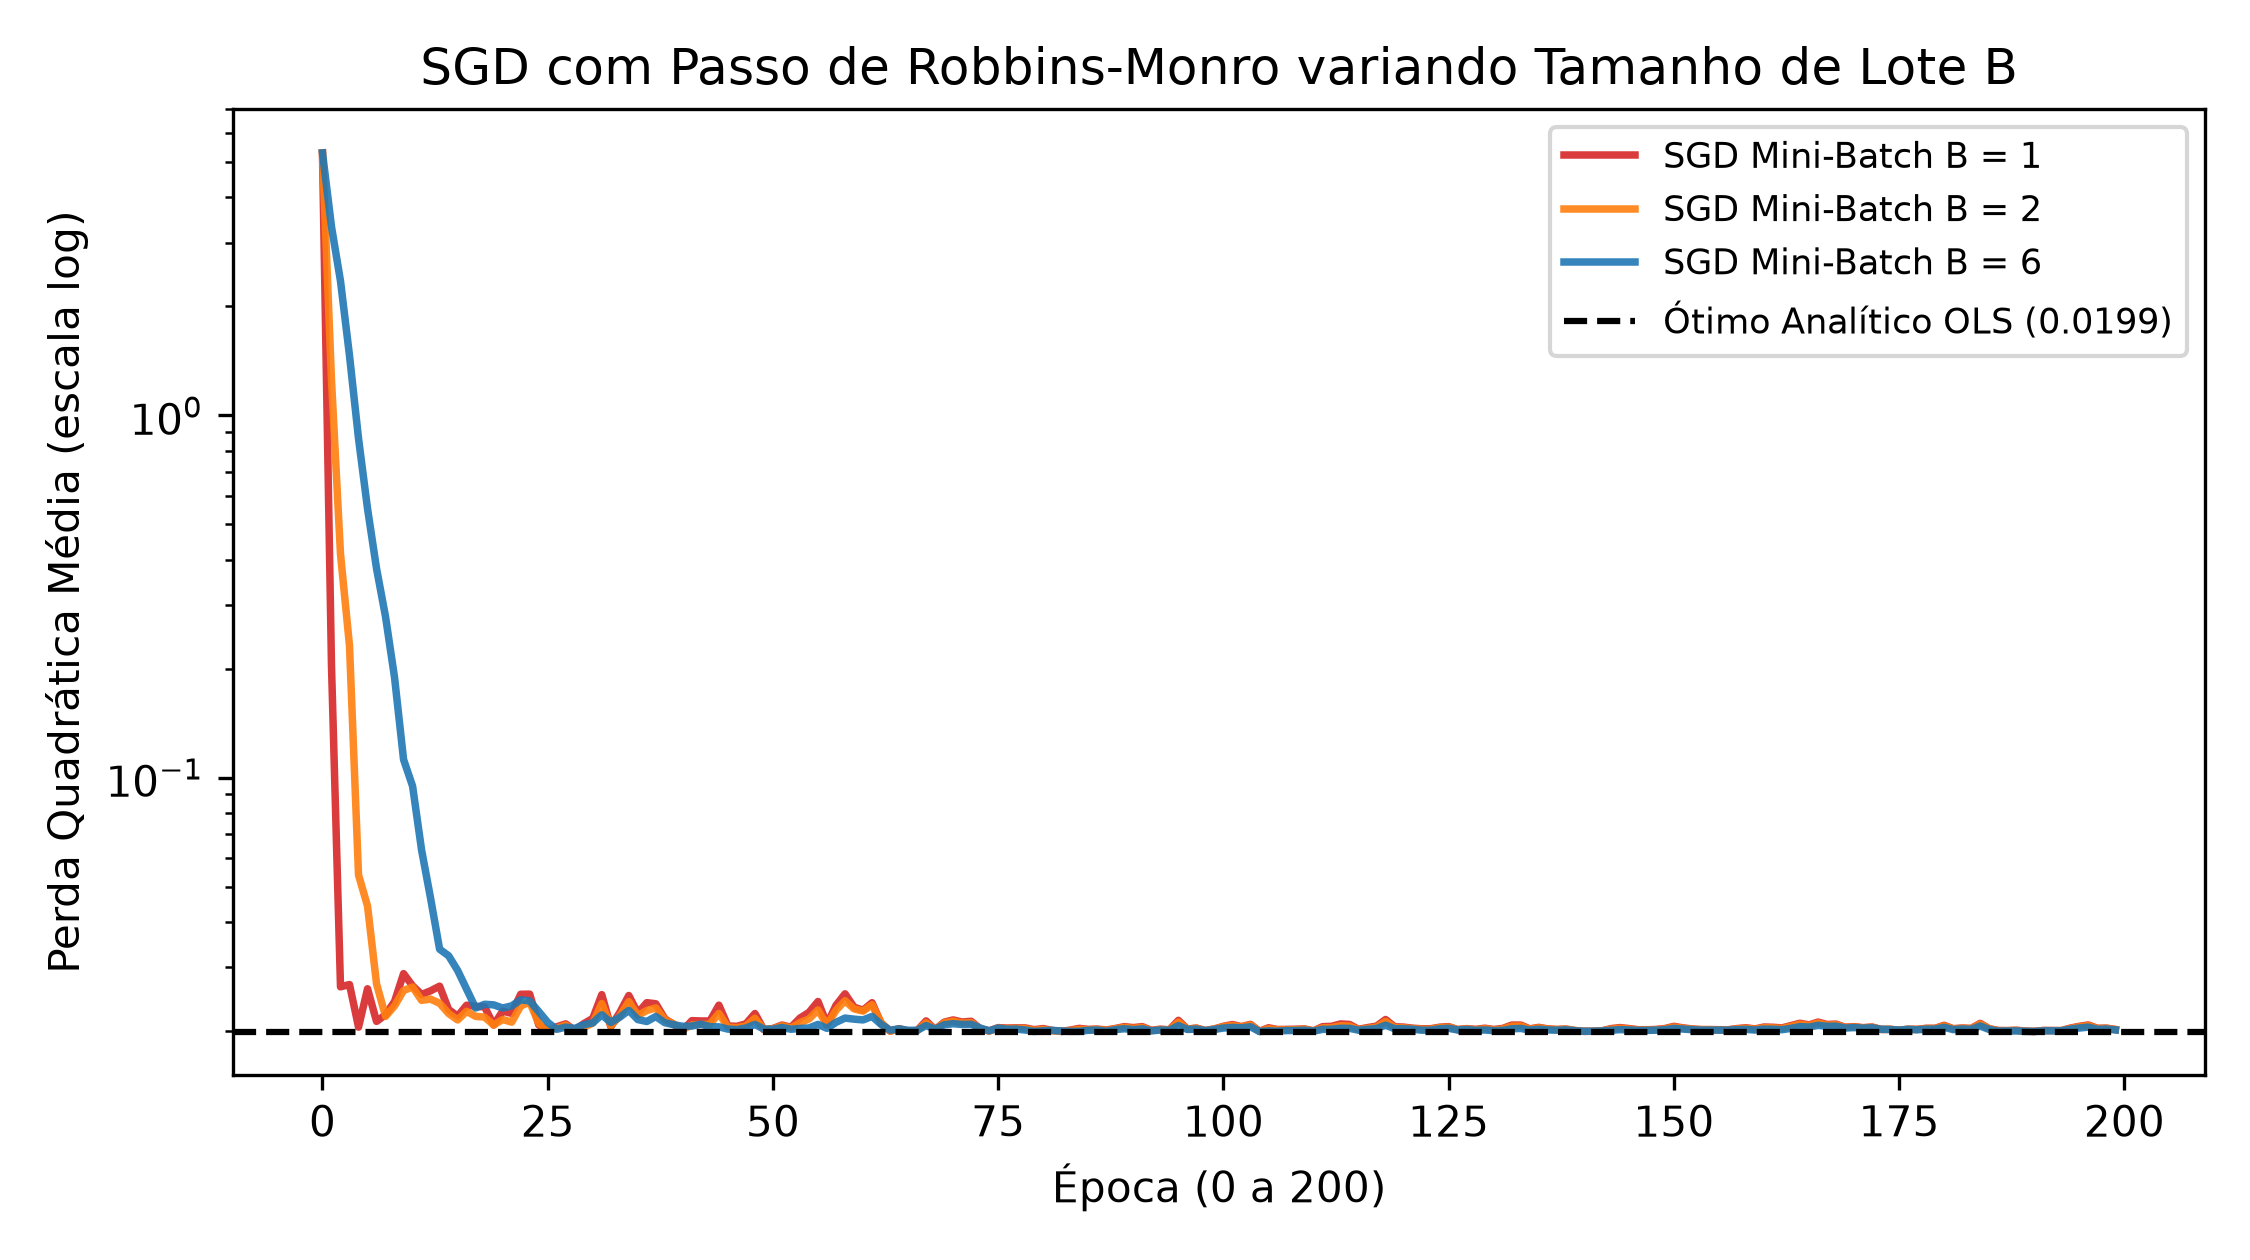
\includegraphics[width=0.78\textwidth]{../figures/q6_minibatch_sgd_robbins_monro.png}
\caption{SGD com passo de Robbins--Monro para tamanhos de lote $B \in \{1, 2, 6\}$.}
\end{figure}

\begin{figure}[H]
\centering
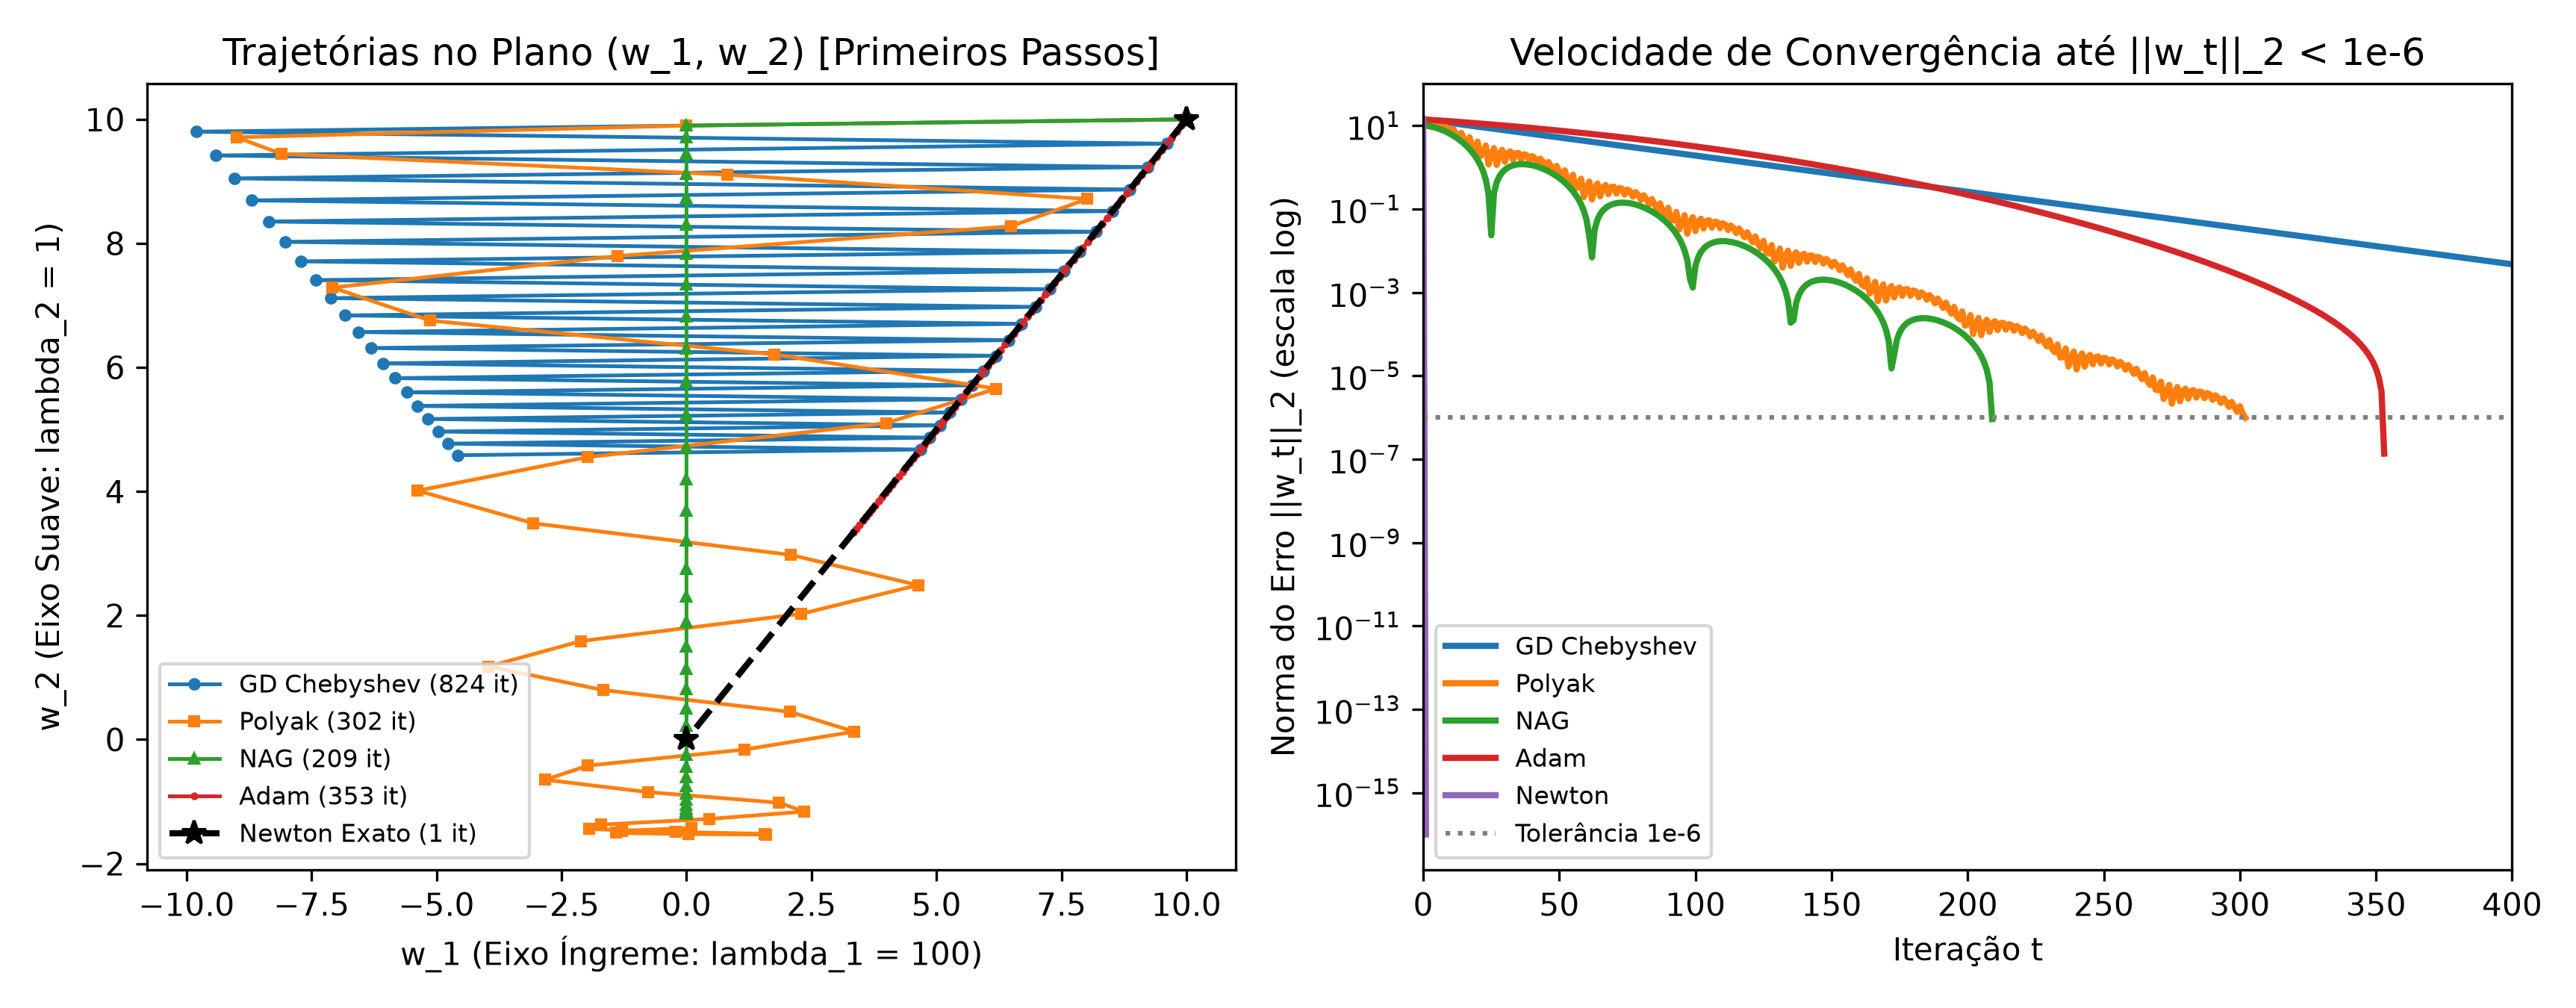
\includegraphics[width=0.92\textwidth]{../figures/q6_quadratica_trajetorias_otimizadores.png}
\caption{Trajetórias e velocidade de convergência na superfície quadrática mal condicionada ($\kappa=100$).}
\end{figure}

% ==============================================================================
\newpage
\section{Questão Bônus: Otimização Não-Suave e ISTA/FISTA}
% ==============================================================================

Para $F(\mathbf{w}) = f(\mathbf{w}) + g(\mathbf{w}) = \frac{1}{2}\|\mathbf{X}\mathbf{w}-\mathbf{y}\|_2^2 + \lambda\|\mathbf{w}\|_1$, um subgradiente $\mathbf{s} \in \partial g(\mathbf{w})$ satisfaz $g(\mathbf{z}) \ge g(\mathbf{w}) + \mathbf{s}^T(\mathbf{z}-\mathbf{w})$, $\forall \mathbf{z}$. Para $|x|$, temos $\partial|x| = \{+1\}$ ($x>0$), $\{-1\}$ ($x<0$) e $[-1, 1]$ ($x=0$), e a condição de Fermat é $\mathbf{0} \in \nabla f(\mathbf{w}^*) + \partial g(\mathbf{w}^*)$.

O operador proximal $\operatorname{prox}_{\gamma g}(\mathbf{v}) = \arg\min_{\mathbf{w}}\{\lambda\|\mathbf{w}\|_1 + \frac{1}{2\gamma}\|\mathbf{w}-\mathbf{v}\|_2^2\}$ desacopla-se em $d$ problemas 1D cuja condição $0 \in \lambda\partial|w_i^*| + \frac{1}{\gamma}(w_i^*-v_i)$ produz o \textit{soft-thresholding}:
\[
w_i^* = \mathcal{S}_{\gamma\lambda}(v_i) = \operatorname{sign}(v_i)\max(|v_i| - \gamma\lambda, 0).
\]
Sempre que $|v_i| \le \gamma\lambda$, o limiar zera exatamente $w_i^* = 0$ (ao contrário do encolhimento linear $\frac{v_i}{1+\gamma\lambda}$ da penalidade $\ell_2$). Minimizando o majorante quadrático de $f$ com constante $L_f = \lambda_{\max}(\mathbf{X}^T\mathbf{X})$, obtém-se o ISTA $\mathbf{w}_{t+1} = \mathcal{S}_{\lambda/L_f}(\mathbf{w}_t - \frac{1}{L_f}\mathbf{X}^T(\mathbf{X}\mathbf{w}_t-\mathbf{y}))$ ($\mathcal{O}(1/t)$), enquanto o FISTA adiciona extrapolação de Nesterov atingindo $\mathcal{O}(1/t^2)$. No problema sintético ($N=50, d=10$, $\mathbf{w}_{\text{true}} = [3{,}0, -2{,}0, 1{,}5, 0, \dots, 0]^T$, $\lambda=5{,}0$), o ISTA recupera o suporte $\{0, 1, 2\}$ com $100\%$ de precisão, zerando rigorosamente os 7 coeficientes ruidosos.

\begin{figure}[H]
\centering
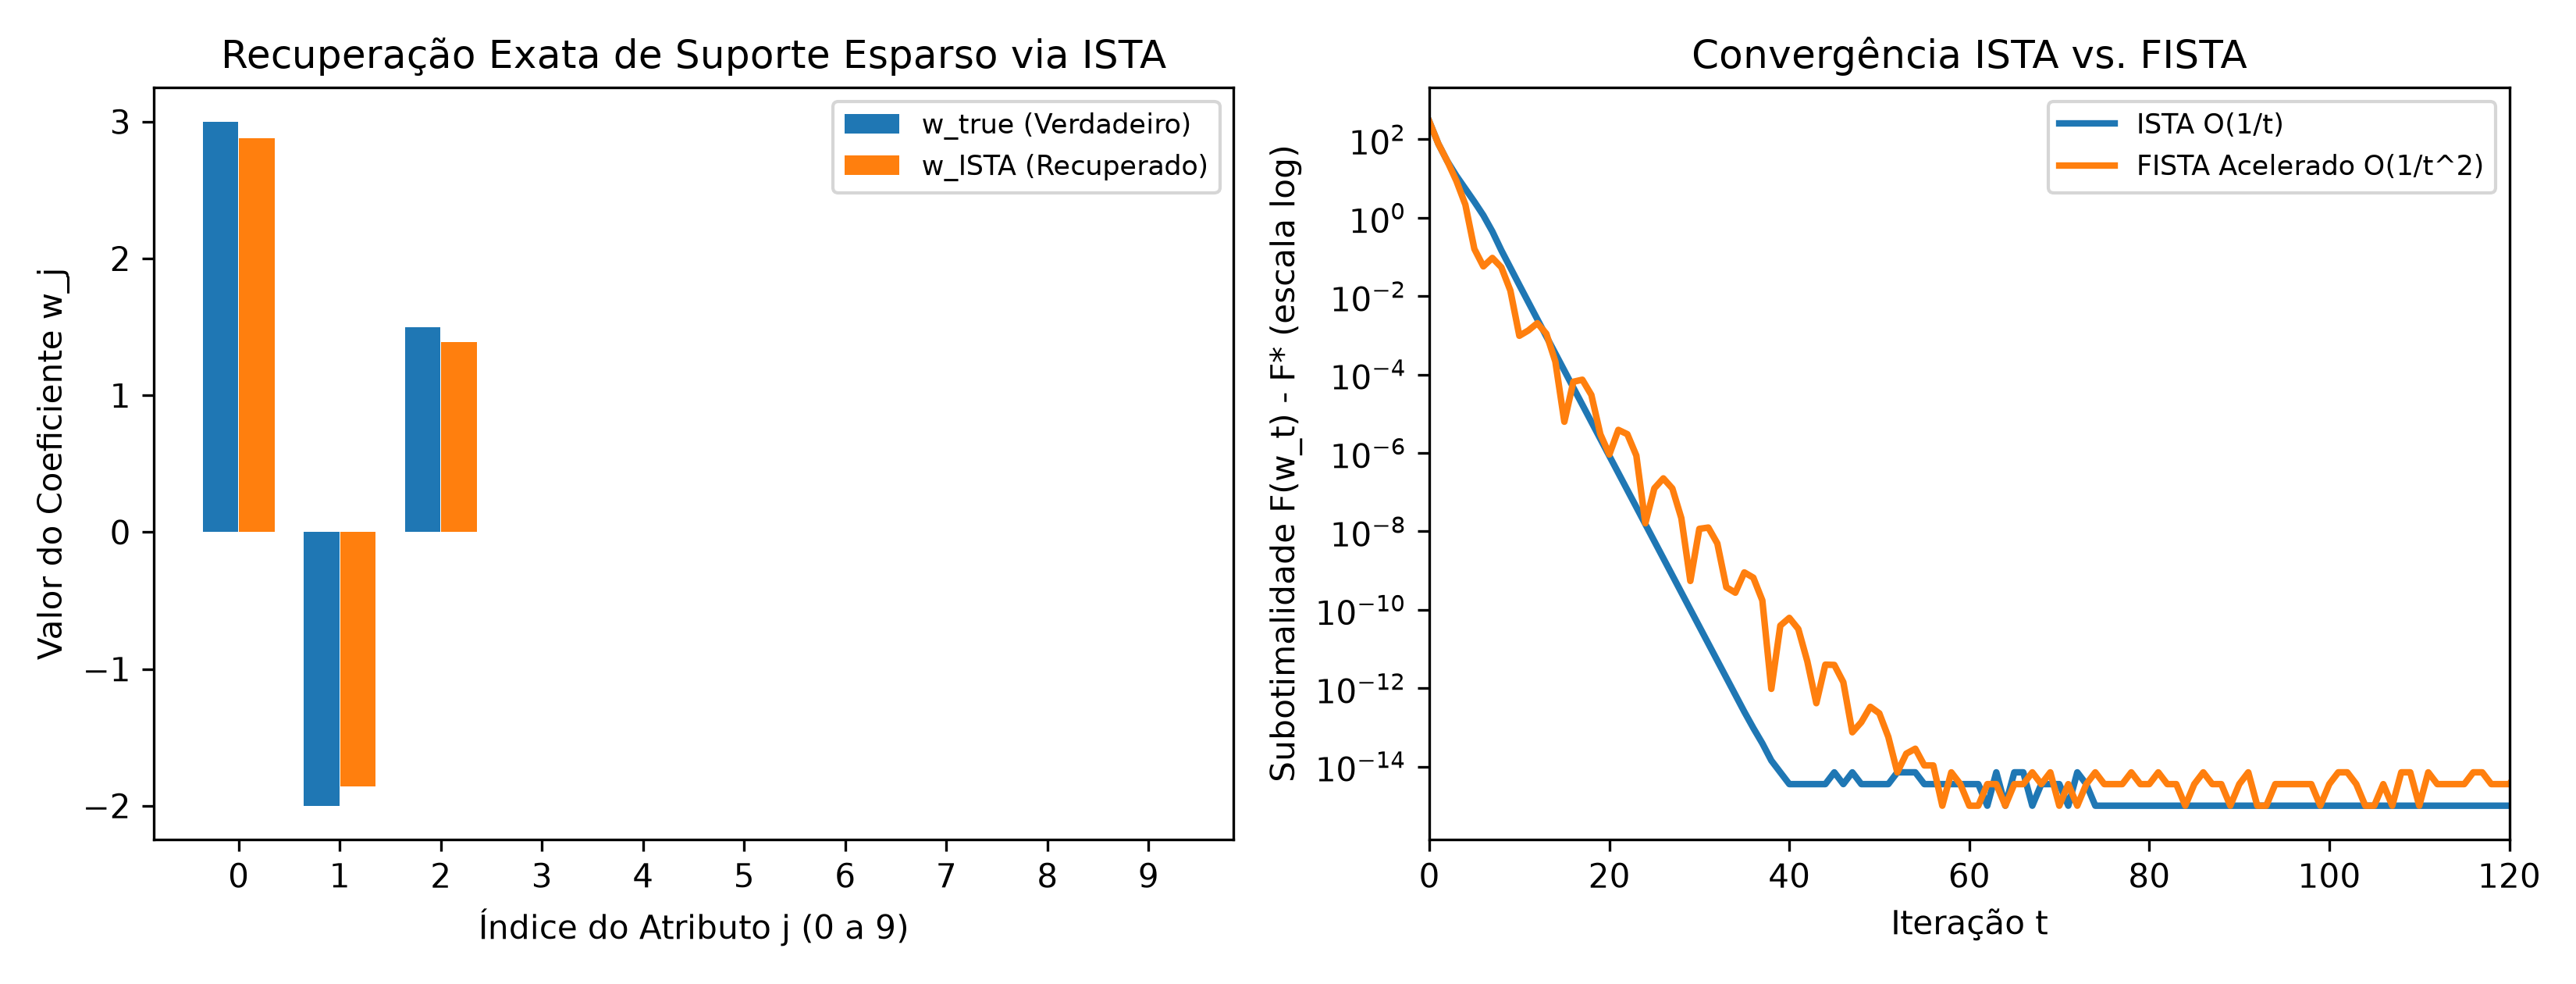
\includegraphics[width=0.92\textwidth]{../figures/qbonus_ista_fista_esparsidade.png}
\caption{Recuperação exata do suporte esparso pelo ISTA e comparação de convergência com o FISTA.}
\end{figure}

\end{document}
